\section{Simulation}

Das folgende Kapitel beschreibt alle Simulationen und deren Auswertungen, die mit den Simu-lation-Tools Matlab und Plecs durchgeführt wurden. Anhand der Resultate konnten die zwei Verfahren miteinander vergleichen und auf ihre Richtigkeit geprüft werden. Mit den Simulationen konnten, erste Einblicke in das Verhalten der beiden Steuerungsverfahren, Phasenanschnitt- und Schwingungspaketsteuerung, gewonnen werden.

\subsection{Simulation mit Matlab}
Um die einphasige Plecs-Simulationen der Phasenanschnitt- und Schwingungspaketsteuerung zu verifizieren, errechnete man parallel zur Plecs-Simulation die gleichen Verfahren mit Matlab. Im folgenden Abschnitt ist aufgezeigt, wie die Ergebnisse der Matlabfunktionen zustande gekommen sind und welche Überlegungen vorgenommen wurde.  




Als erstes simulierte man eine periodische Sinusfunktion im Zeitbereich mit verschiedenen Phasenanschnittenswinkeln. Die Periodenlänge definierte man dabei auf 2$\pi$ und die Amplitude des Sinus beträgt $\pm$ \SI{1}{Volt}. Der Winkel des Phasenanschnittes wurde mit verschieden, geläufigen Werte wie zum Beispiel 30\textdegree, 45\textdegree, 60\textdegree, 90\textdegree oder 120\textdegree betrachtet. In den folgenden Bildern \ref{fig:eingangssignal_mit_Matlab} erkennt man die Sinusfunktionen mit einem Phasenanschnitt von $60^\circ$ in Abbildung \ref{fig:Einganssignal 60} und \ref{fig:Einganssignal 90} $90^\circ$ in der Grafik \ref{fig:Einganssignal 90}. Weitere Funktionen mit den anderen Anschnittswinkeln sind im Anhang ersichtlich.
 

\begin{figure}[h]
	\centering
	\subfloat[][]{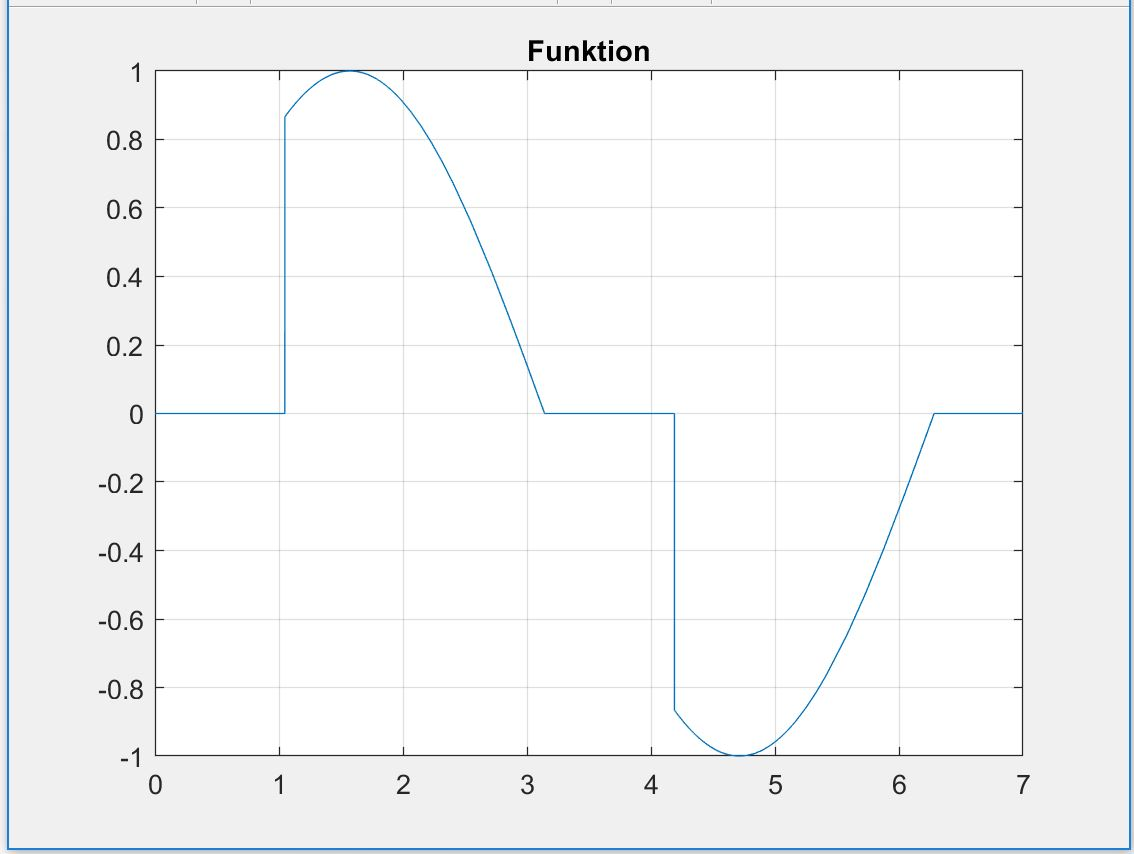
\includegraphics[width=0.47\linewidth]{eingangssignal_60.png}\label{fig:Einganssignal 60}}\qquad
	\subfloat[][]{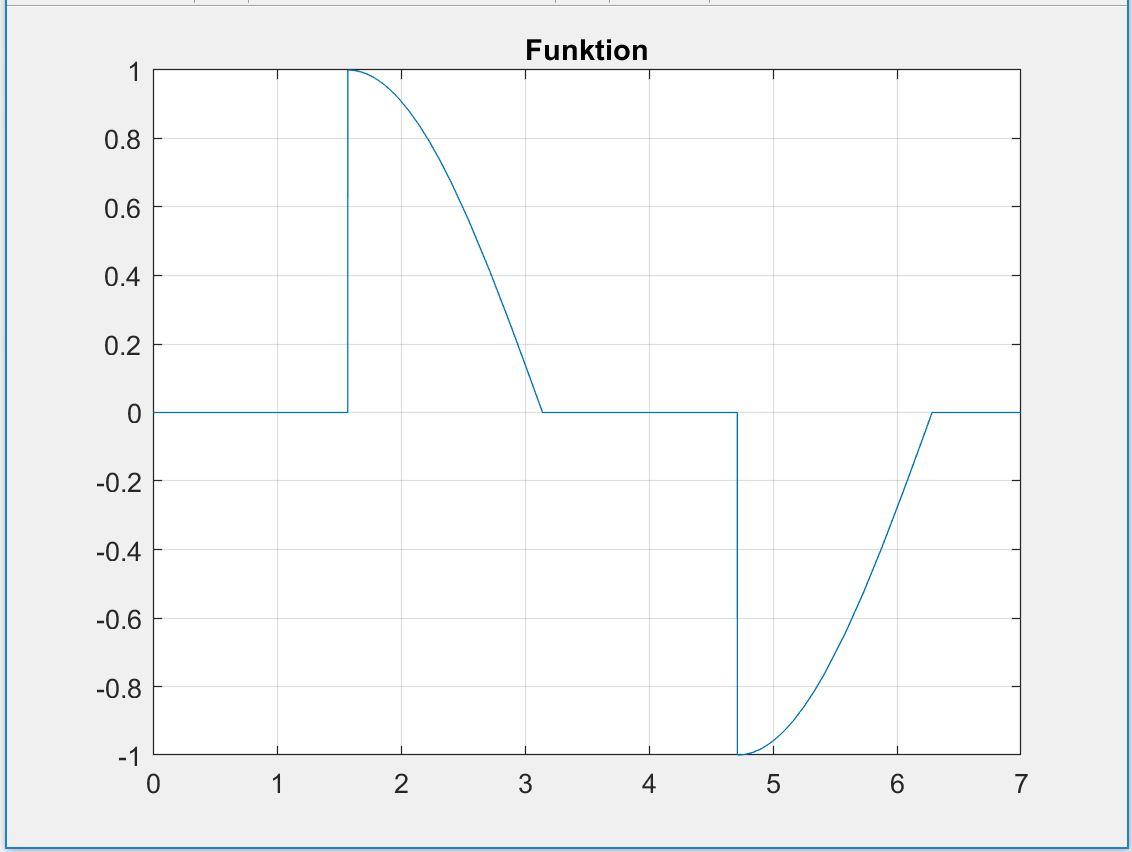
\includegraphics[width=0.47\linewidth]{eingangssignal_90.png}\label{fig:Einganssignal 90}}
	\caption{Einganssignal mit Phasenanschnitt (a) $60^\circ$ (b) $90^\circ$}
	\label{fig:eingangssignal_mit_Matlab}
\end{figure} 

Als nächstes zerlegte man die Funktionen in die verschiedenen Frequenzanteile. Dies wird auch als Fourier-Analyse bezeichnet. Mit Hilf der Fourier-Koeffizienten $a\textsubscript{0}$, $b\textsubscript{n}$ und $a\textsubscript{n}$ konnte das Amplituden und Phasenspektrum berechnet werden. Die mathematische Formel der Koeffizienten, der Spektren und die Beschreibung der Fourier-Analyse ist in Kapitel \ref{sec:Verzerrte_Schwingung} aufgezeigt.
  
\newpage
Die Darstellung im Zeitbereich beziehungsweise im Frequenzbereich sind äquivalent, sie enthalten also beide die vollständige Information über die Funktionen. Im Frequenzspektrum benutzt man die vertikalen Linien, um die Komponenten der einzelnen Frequenzen auf der x-Achse anzugeben. Die y-Achse zeigt die Länge der Amplitude, bei den verschiedenen x-Werten, an. In den untenstehenden Grafiken \ref{fig:Amplituden- und Phasenspektrum} erkennt man das Amplituden- und Phasenspektrum des in Abbildung \ref{fig:eingangssignal_mit_Matlab} dargestellten Signale.

\begin{figure}[h]
	\centering
	\subfloat[][]{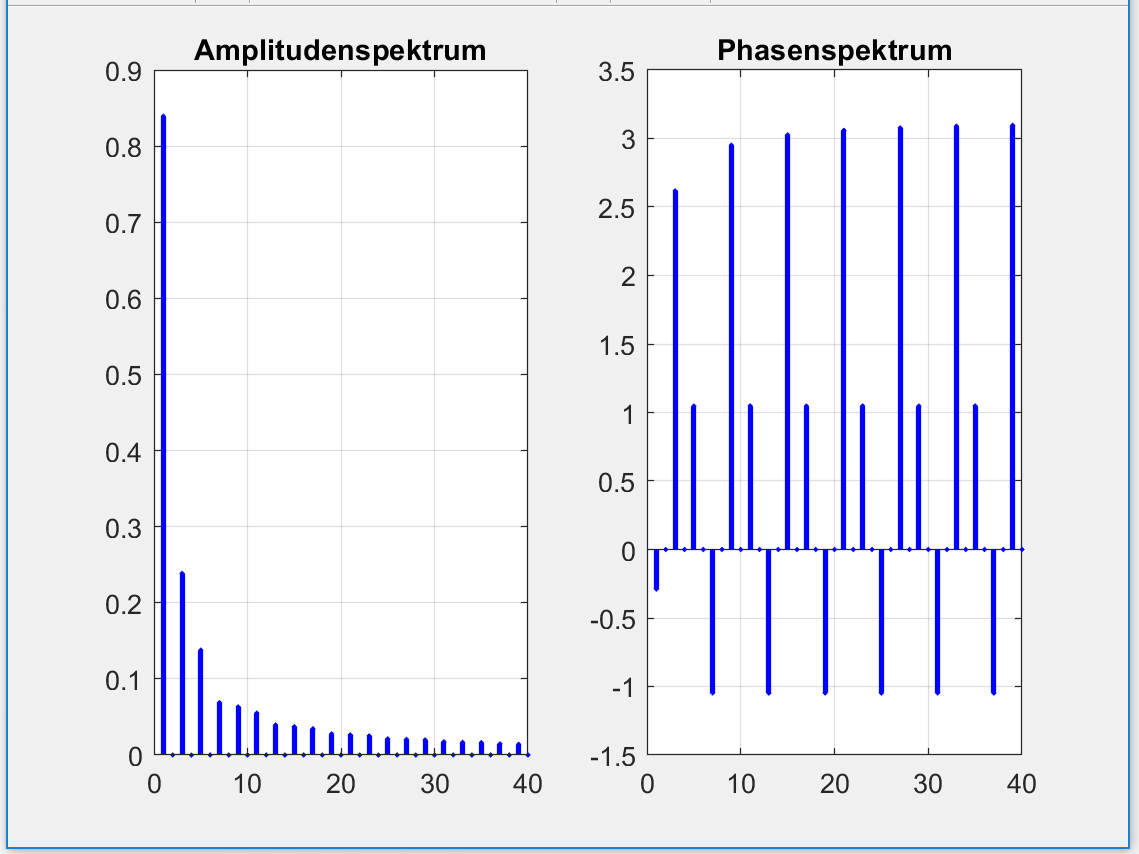
\includegraphics[width=0.47\linewidth]{A_PH_60.png}\label{fig:Amplituden- und Phasenspektrum 60}}\qquad
	\subfloat[][]{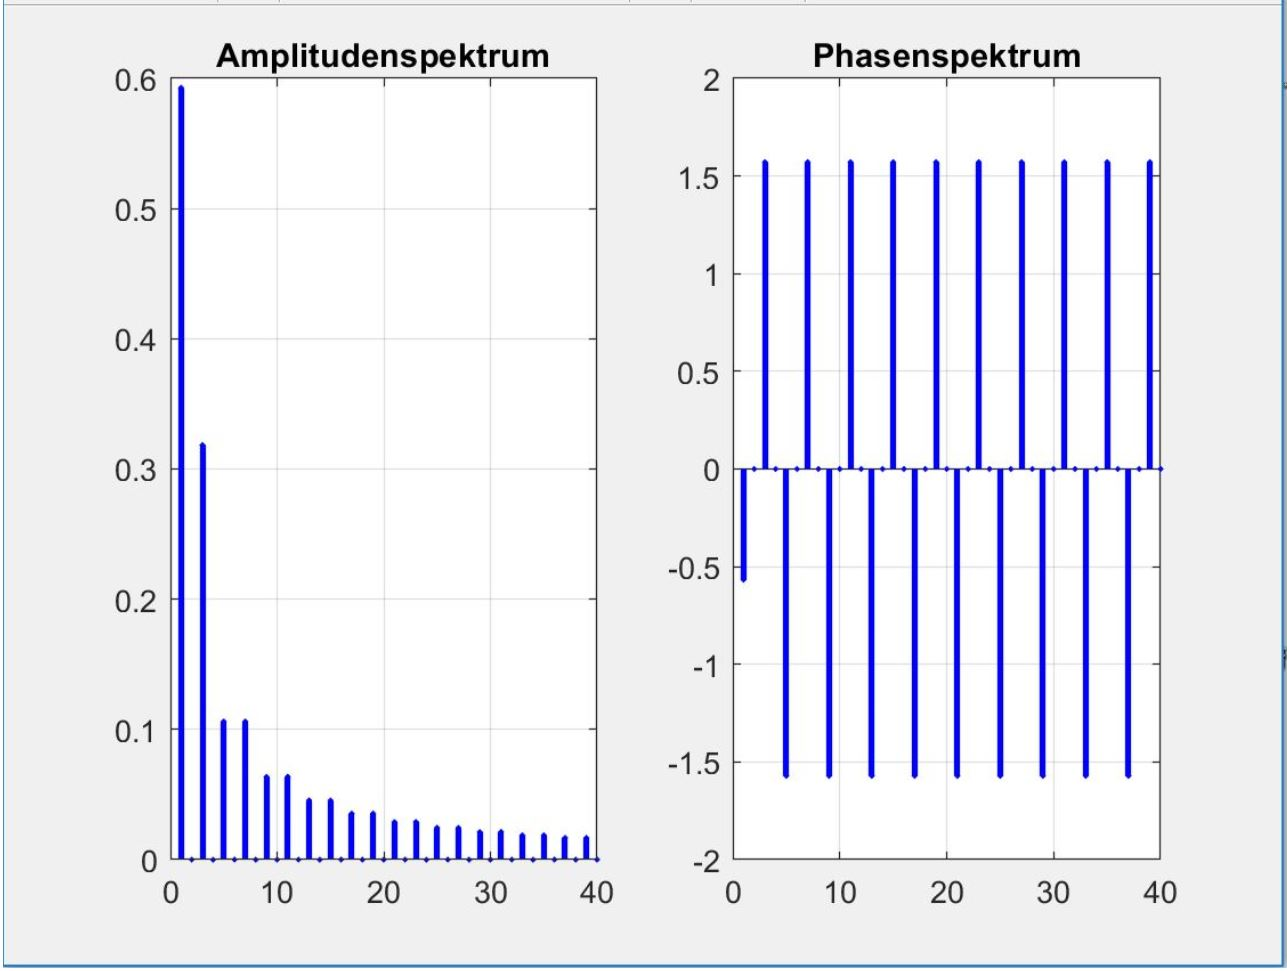
\includegraphics[width=0.47\linewidth]{A_PH_90.png}\label{fig:Amplituden- und Phasenspektrum 90}}
	\caption{Amplituden- und Phasenspektrum (a) $60^\circ$ (b) $90^\circ$}
	\label{fig:Amplituden- und Phasenspektrum}
\end{figure} 

Zur Kontrolle der Berechnungen des Amplituden- und Phasenspektrum, wurde mit den zwei Spektren das Eingangssignal rekonstruierte. Die Signale sind auf der nächsten Abbildung \ref{fig:Rekonstruiertes Signal} erkennbar. Es ist ersichtlich das die Rundung des Sinus nicht genau dem, des eigentlichen Signals entspreche \ref{fig:eingangssignal_mit_Matlab}. Dies kommt davon, dass man die Funktion in «nur» 40 Frequenzanteile unterteilt hat. Würde man eine höhere Anzahl Anteile verwenden, so könnte das Rauschen deutlich verkleinert werden. Da man jedoch nur einen ungefähren Vergleich der beiden Funktionen haben möchte, reicht diese Anzahl völlig aus. 

\begin{figure}[h]
	\centering
	\subfloat[][]{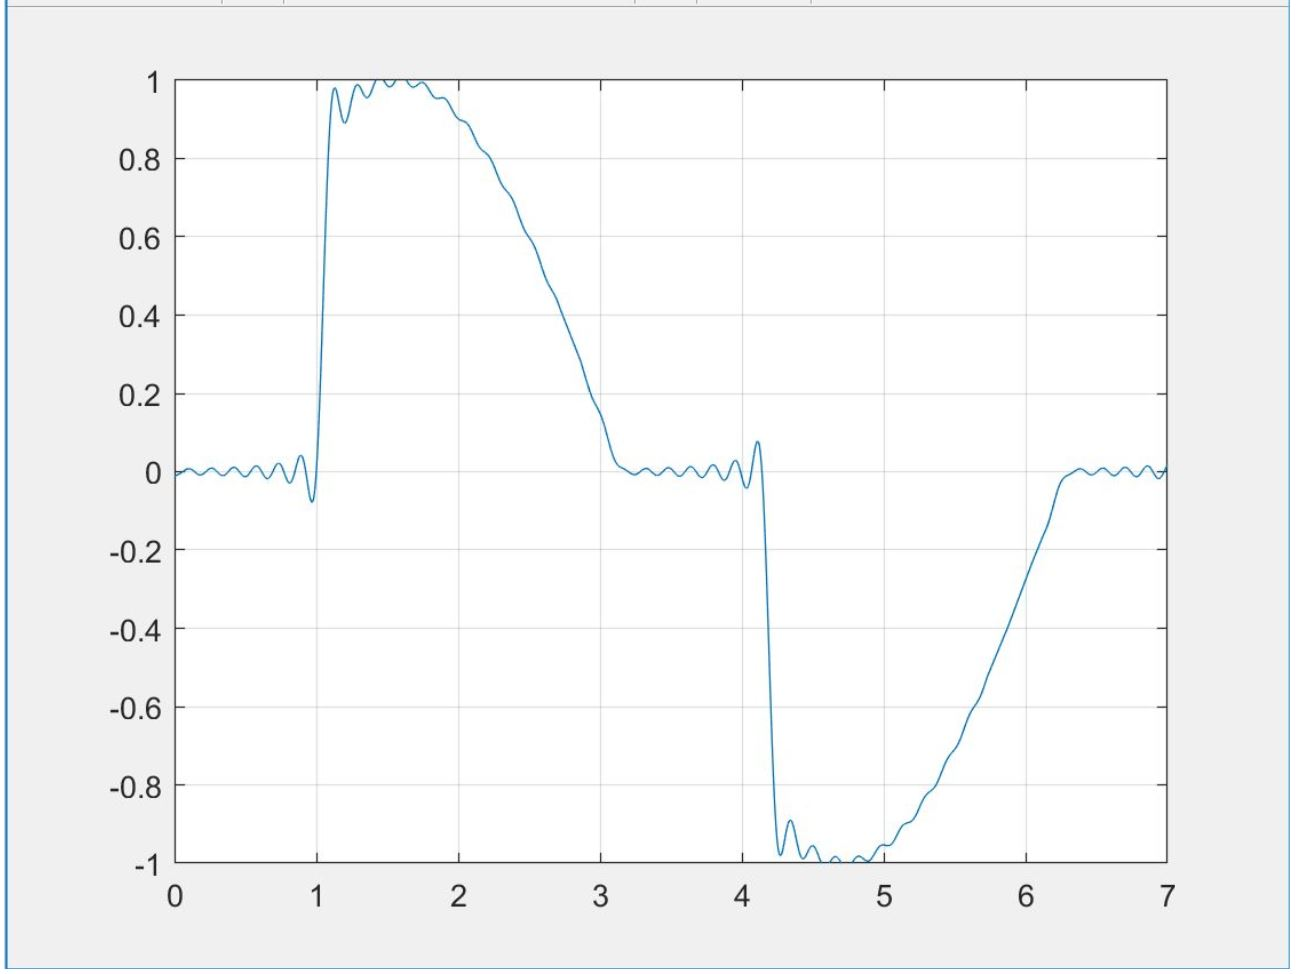
\includegraphics[width=0.47\linewidth]{re_eingangssignal_60.png}\label{fig:rekonstruiertes Signal 60}}\qquad
	\subfloat[][]{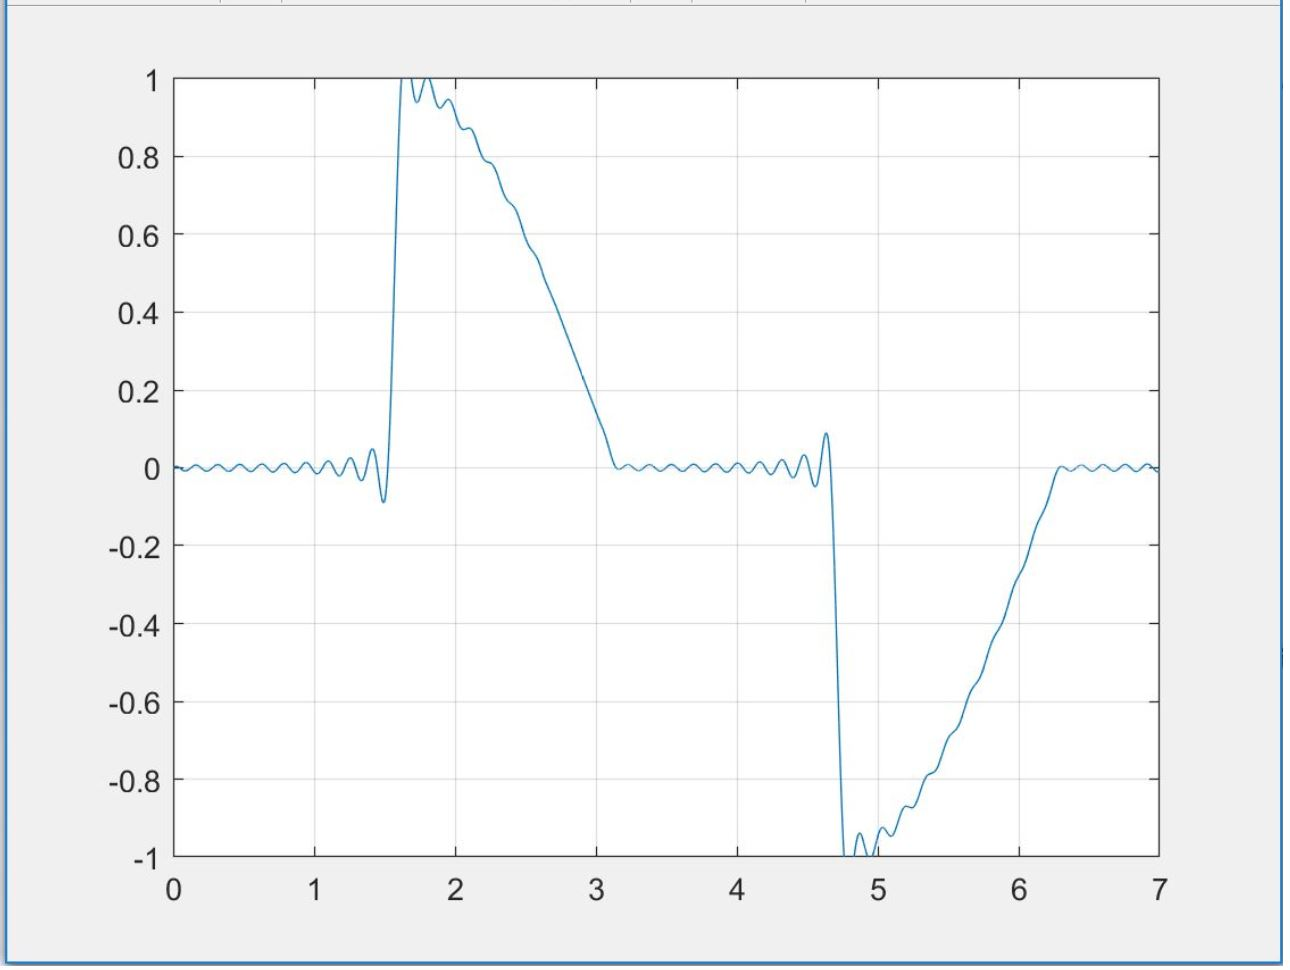
\includegraphics[width=0.47\linewidth]{re_einganssignal_90.png}\label{fig:rekonstruiertes Signal 90}}
	\caption{Rekonstruiertes Signal (a) $60^\circ$ (b) $90^\circ$}
	\label{fig:Rekonstruiertes Signal}
\end{figure} 


Nach dem man das Phasenanschnittsignal, das Amplitudenspektrum,  das Phasenspektrum und das rekonstruierende Eingangssignal von Hand berechnet und dargestellt hat, überprüfte man mit Hilfe der FFT-Funktion (Fast Fourier Transform) von Matlab die Werte der Grafiken. In der folgenden Abbildung \ref{fig:FFT mit Matlab} erkennt man die Plots bei einem Winkel von $60^\circ$. Bei dem Amplituden- und Phasenspektrum wurde die x-Achse so normiert, dass die Werte ein Vielfaches der Grundfrequenz von 50 Hz sind. So ist zum Beispiel der Wert bei 500 beim FTT zu vergleichen mit dem Wert 10 bei den von Hand berechneten Spektren. Als Resultat erkennt man das beide Methoden die gleichen Ergebnisse herausgeben haben. Es kann davon ausgegangen werden, dass die Überlegung der  Berechnungen korrekt waren.

\begin{figure}[ht!]
	\centering
	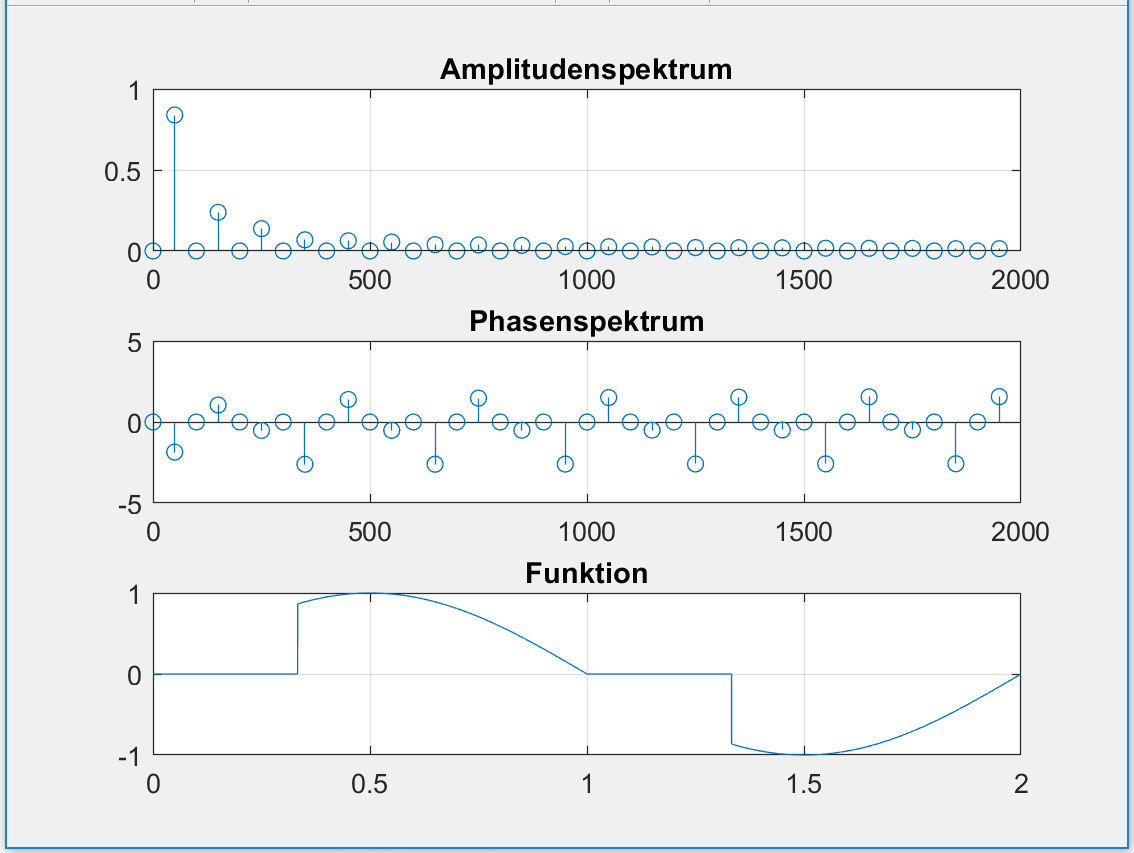
\includegraphics[scale=0.7]{FFT_mit_Matlab.png}	
	\caption{FFT mit der Matlabfunktion dargestellt}
	\label{fig:FFT mit Matlab}
\end{figure}

Bei der zweiten Funktion, die zu überprüfen, und simulieren war, handelte es sich um eine Schwingungspaketsteuerung. Die komplette Paketdauer beträgt bei den abgebildeten Funktionen 20 Halbwellen \ref{fig:Schwingungspaket Matlab}. Es wurden nun verschiedene Einschaltverfahren untersucht. In der Abbildung \ref{fig:Schwingungspaket Matlab} erkennt man im linken Bild \ref{fig:Schwingungspacket 0.5} einen duty cycle von 0.5. Demzufolge sind immer 10 Halbwellen ausgeschaltet und die anderen 10 eingeschlatet.
Auf der rechten Seite \ref{fig:Schwingungspacket 0.8} beträgt der Wert des duty cycle 0.8. Es sind also zuerst 4 Halbwellen ausgeschaltet und die restlichen 16 Halbwellen werden angesteuert. Für einen sinnvollen Vergleich untersuchte man bei beiden Simulationsmethoden 5 komplette Schwingungspakete.

\begin{figure}[ht!]
	\centering
	\subfloat[][]{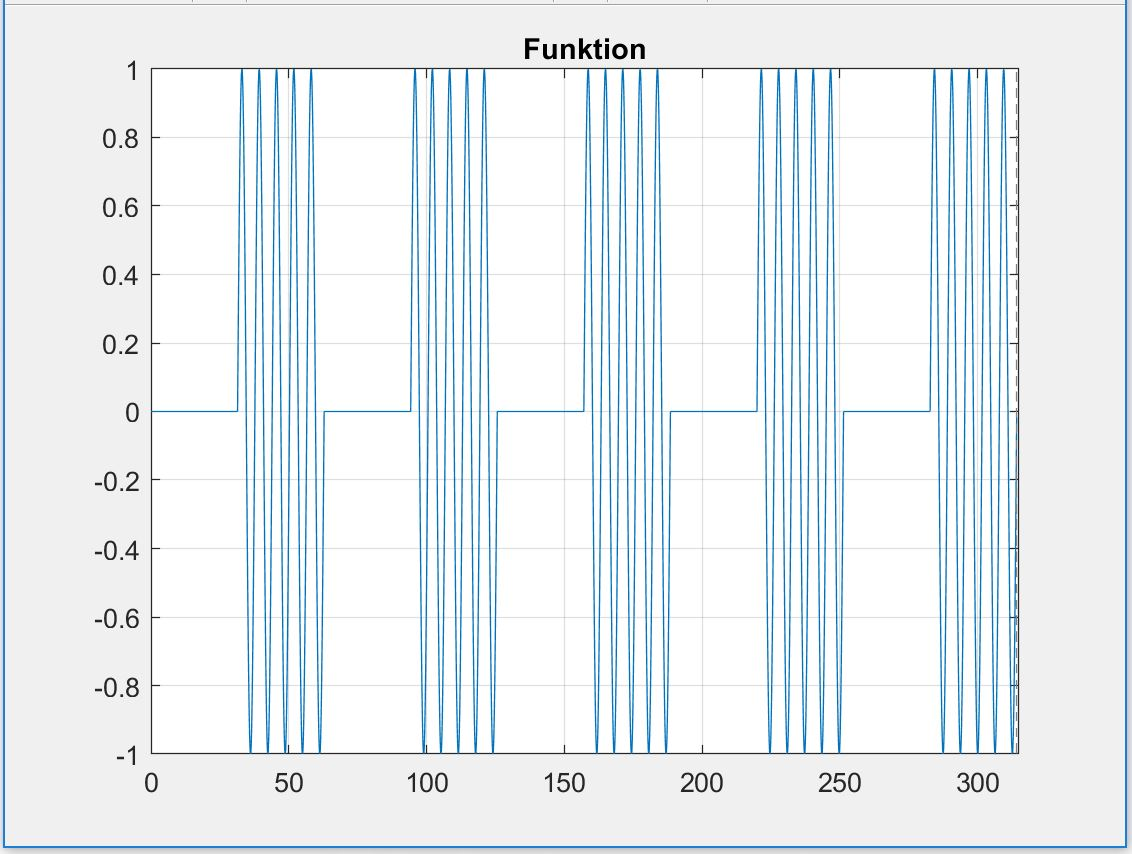
\includegraphics[width=0.45\linewidth]{Schwingungspaket_0_5.png}\label{fig:Schwingungspacket 0.5}}\qquad
	\subfloat[][]{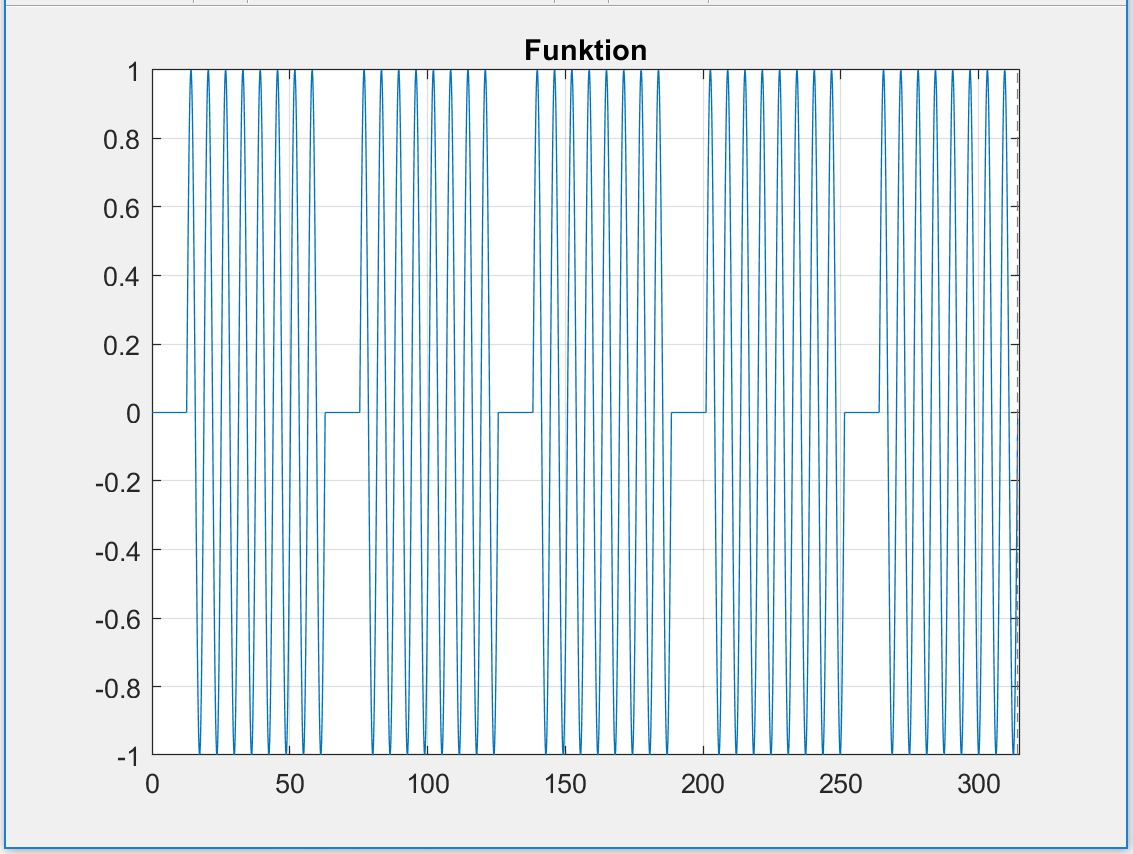
\includegraphics[width=0.45\linewidth]{Schwingungspaket_0_8.png}\label{fig:Schwingungspacket 0.8}}
	\caption{Schwingungspaket mit einem duty cycle von (a) 0.5 (b) 0.8}
	\label{fig:Schwingungspaket Matlab}
\end{figure} 

Um auch hier die Plecs-Simulation zu überprüfen, stellte man das Amplitudenspektrum absolut linear dar. Bei der folgenden Abbildungen \ref{fig:Schwingungspaketspektrum Matlab} erkennt man diese Spektren. Interessant sind da vor allem die Subharmonischen Schwingungen, welche sich unterhalb der Grundfrequenz von 50 Hz befinden. Sie sind jeweils auf der linken Seite der  Grafiken veranschaulicht. Damit man alle relevanten Oberschwingungen erkennt, wurde das Spektrum bis auf 1000 Hz erweitert. Dies ist auf der rechten Seite des jeweiligen Bildes ersichtlich. Bei der linken Abbildung \ref{fig:Schwingungspacketspektrum 0.5} wurde das Amplitudenspektrum mit einem duty cycle von 0.5 dargestellt und im rechten Bild \ref{fig:Schwingungspacketspektrum 0.8} verwendete man einen duty cycle von 0.8. Vergleicht man die zwei Diagramme erkennt man, dass je grösser der duty cycle, desto höher ist der Peak-Wert bei der Grundfrequenz von 50 Hz. Dies kommt davon, dass bei einem grösseren duty cycle mehre Sinusschwingungen vorkommen als bei einem niedrigen. 
 

\begin{figure}[ht!]
	\centering
	\subfloat[][]{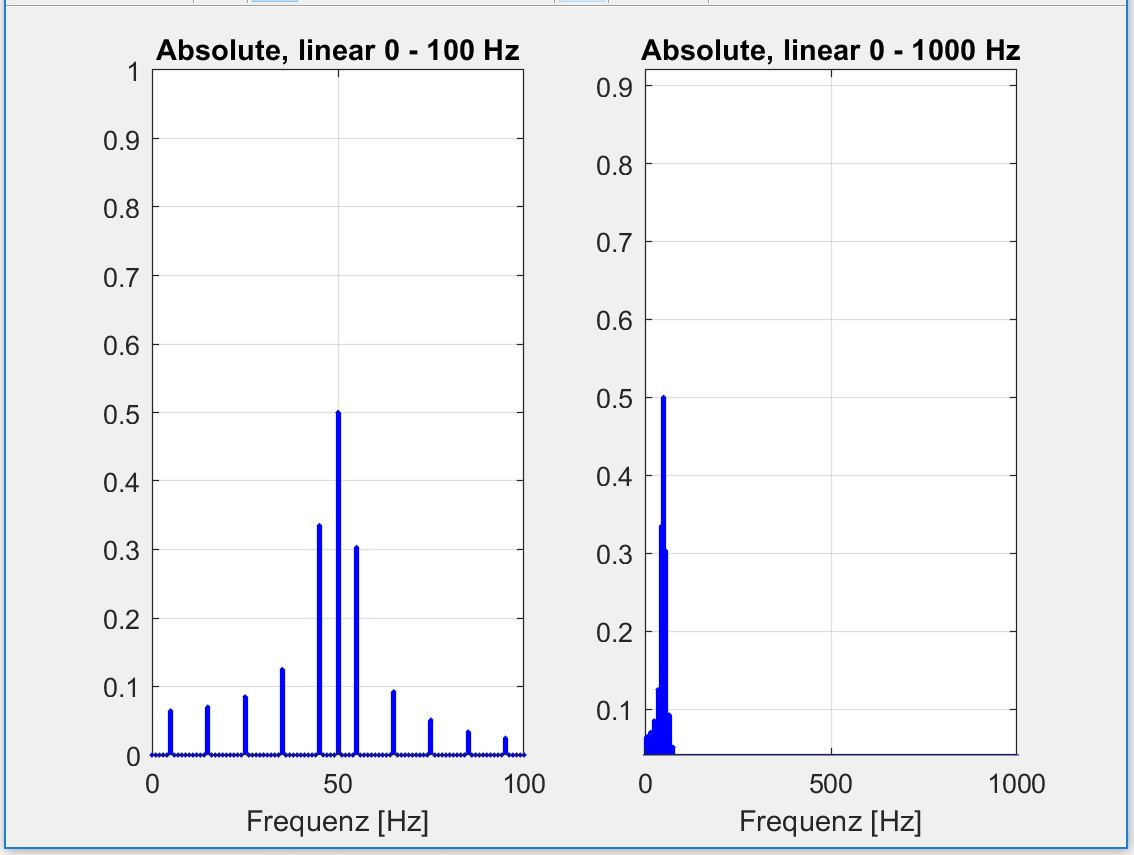
\includegraphics[width=0.45\linewidth]{Oberwellen_0_5.png}\label{fig:Schwingungspacketspektrum 0.5}}\qquad
	\subfloat[][]{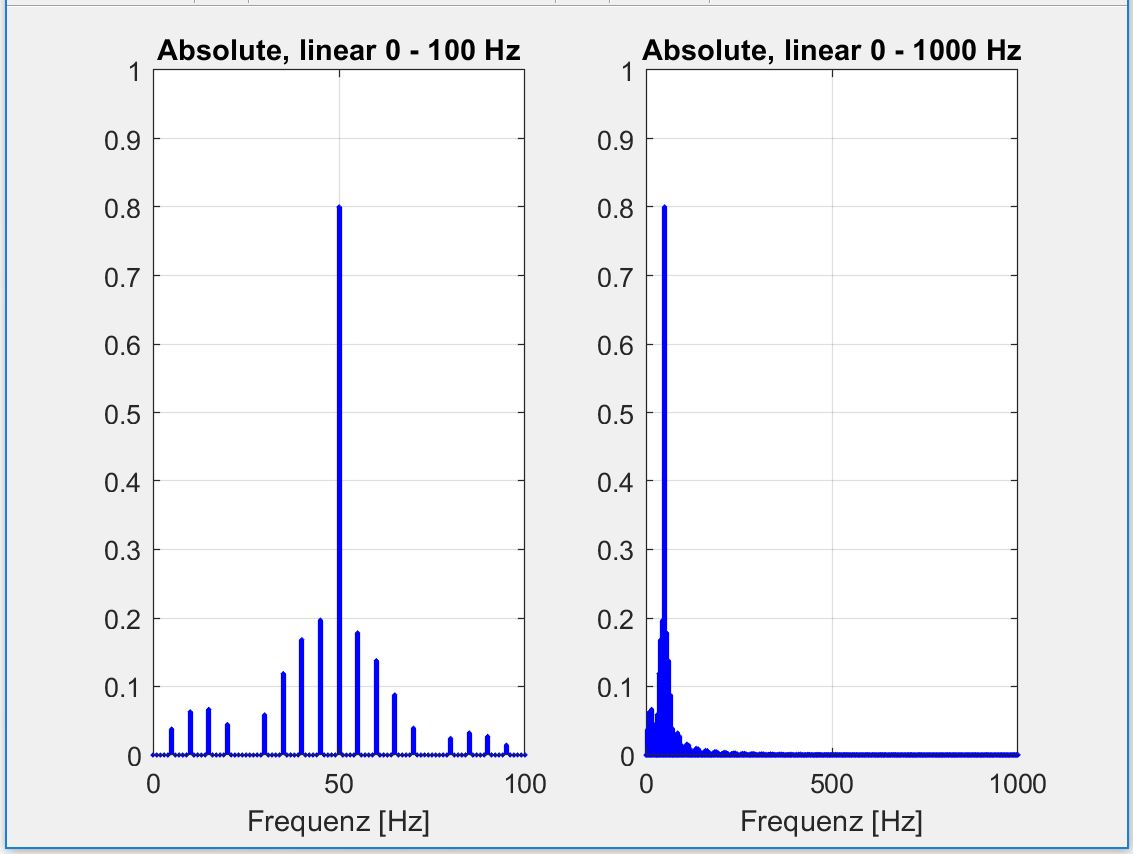
\includegraphics[width=0.45\linewidth]{Oberwellen_0_8.png}\label{fig:Schwingungspacketspektrum 0.8}}
	\caption{Lineares absolutes Spektrum mit einem duty cycle von (a) 0.5 (b) 0.8}
	\label{fig:Schwingungspaketspektrum Matlab}
\end{figure}

Die dritte Darstellungsfunktion, welche man untersuchte, war der absolute Logarithmus. Man erkennt die Darstellung in der Abbildung \ref{fig:absolut_logaritmic_matlab}. Für die Berechnung der Dezibel, verwendete man das Verhältnis der Bezugsspannung U0 bei 50 Hz mit der zu messenden Spannung Un. Auch hier wurden die bereits bekannten duty cycle Werte von 0.5 in der linken Abbildung  \ref{fig:absolut_logarithmic_0.5} und 0.8 in der rechten Grafik \ref{fig:absolut_logarithmic_0.8} verwendet um den absoluten Logarithmus anzuzeigen.



\begin{figure}[ht!]
	\centering
	\subfloat[][]{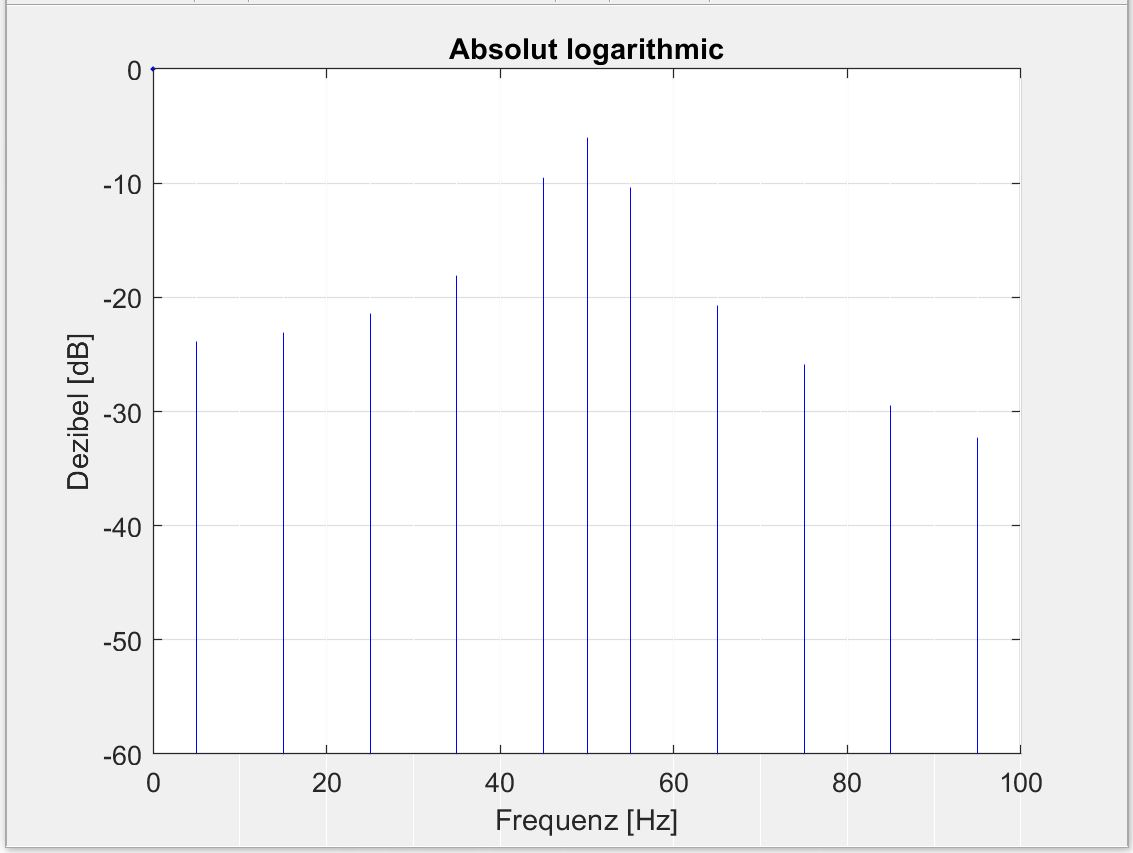
\includegraphics[width=0.45\linewidth]{absolut_logaritmic_0_5.png}\label{fig:absolut_logarithmic_0.5}}\qquad
	\subfloat[][]{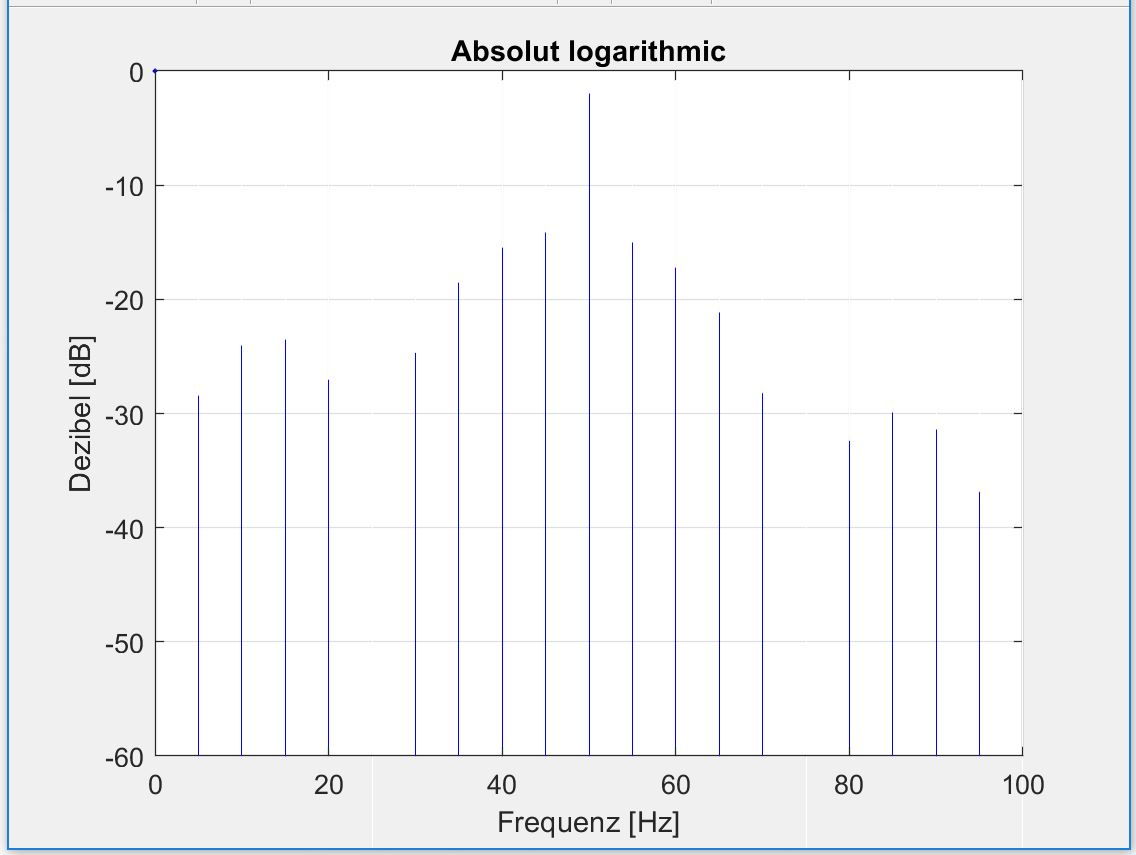
\includegraphics[width=0.45\linewidth]{absolut_logaritmic_0_8.png}\label{fig:absolut_logarithmic_0.8}}
	\caption{Lineares absolutes Spektrum mit einem duty cycle von (a) 0.5 (b) 0.8}
	\label{fig:absolut_logaritmic_matlab}
\end{figure}
\newpage
\subsection{Simulation mit Plecs}

Mit dem Simulationsprogramm Plecs wurden alle gewünschten Ansteuerungen simuliert. Die einphasigen Simulationen der Phasenanschnitt- und der Schwingungspaketsteuerung konnten mit den Matlab-Funktionen verglichen und ausgewertet werden. Nach dem dies verifiziert wurde, stellte man Verfahren für den dreiphasigen Phasenanschnitt- und Schwingungspaketsteuerung her. Ausserdem konstruierte man Kombinationen der beiden Verfahren im einphasigen und dreiphasigen System.\todo{alle Verfahren auflisten} Die Resultate sind auf den folgenden Seiten ersichtlich.\\



Auch bei der Plecs-Simulationen wurde als erstes die Phasenanschnittsteuerung untersucht. Gleich wie bei der Matlab-Simulation konnten die verschiedenen Winkeln des Anschnittes nach Belieben eingestellt werden. Um die Resultate verifizieren zu könne wählte man die selben Winkel wie beim Matlab in der Abbildung \ref{fig:eingangssignal_mit_Matlab}. In der unteren Grafik, erkennt man ein Sinussignal mit einem Phasenanschnitt von $60^\circ$ links \ref{fig:plecs_eingangssignal_60} und einen mit $90^\circ$ rechts \ref{fig:plecs_eingangssignal_90}. Um die Spektren mit den Matlab-Simulationen vergleichen zu können, wurde die Amplitude des Sinussignales auch auf ± 1 Volt gestellt.  

\begin{figure}[ht!]
	\centering
	\subfloat[][]{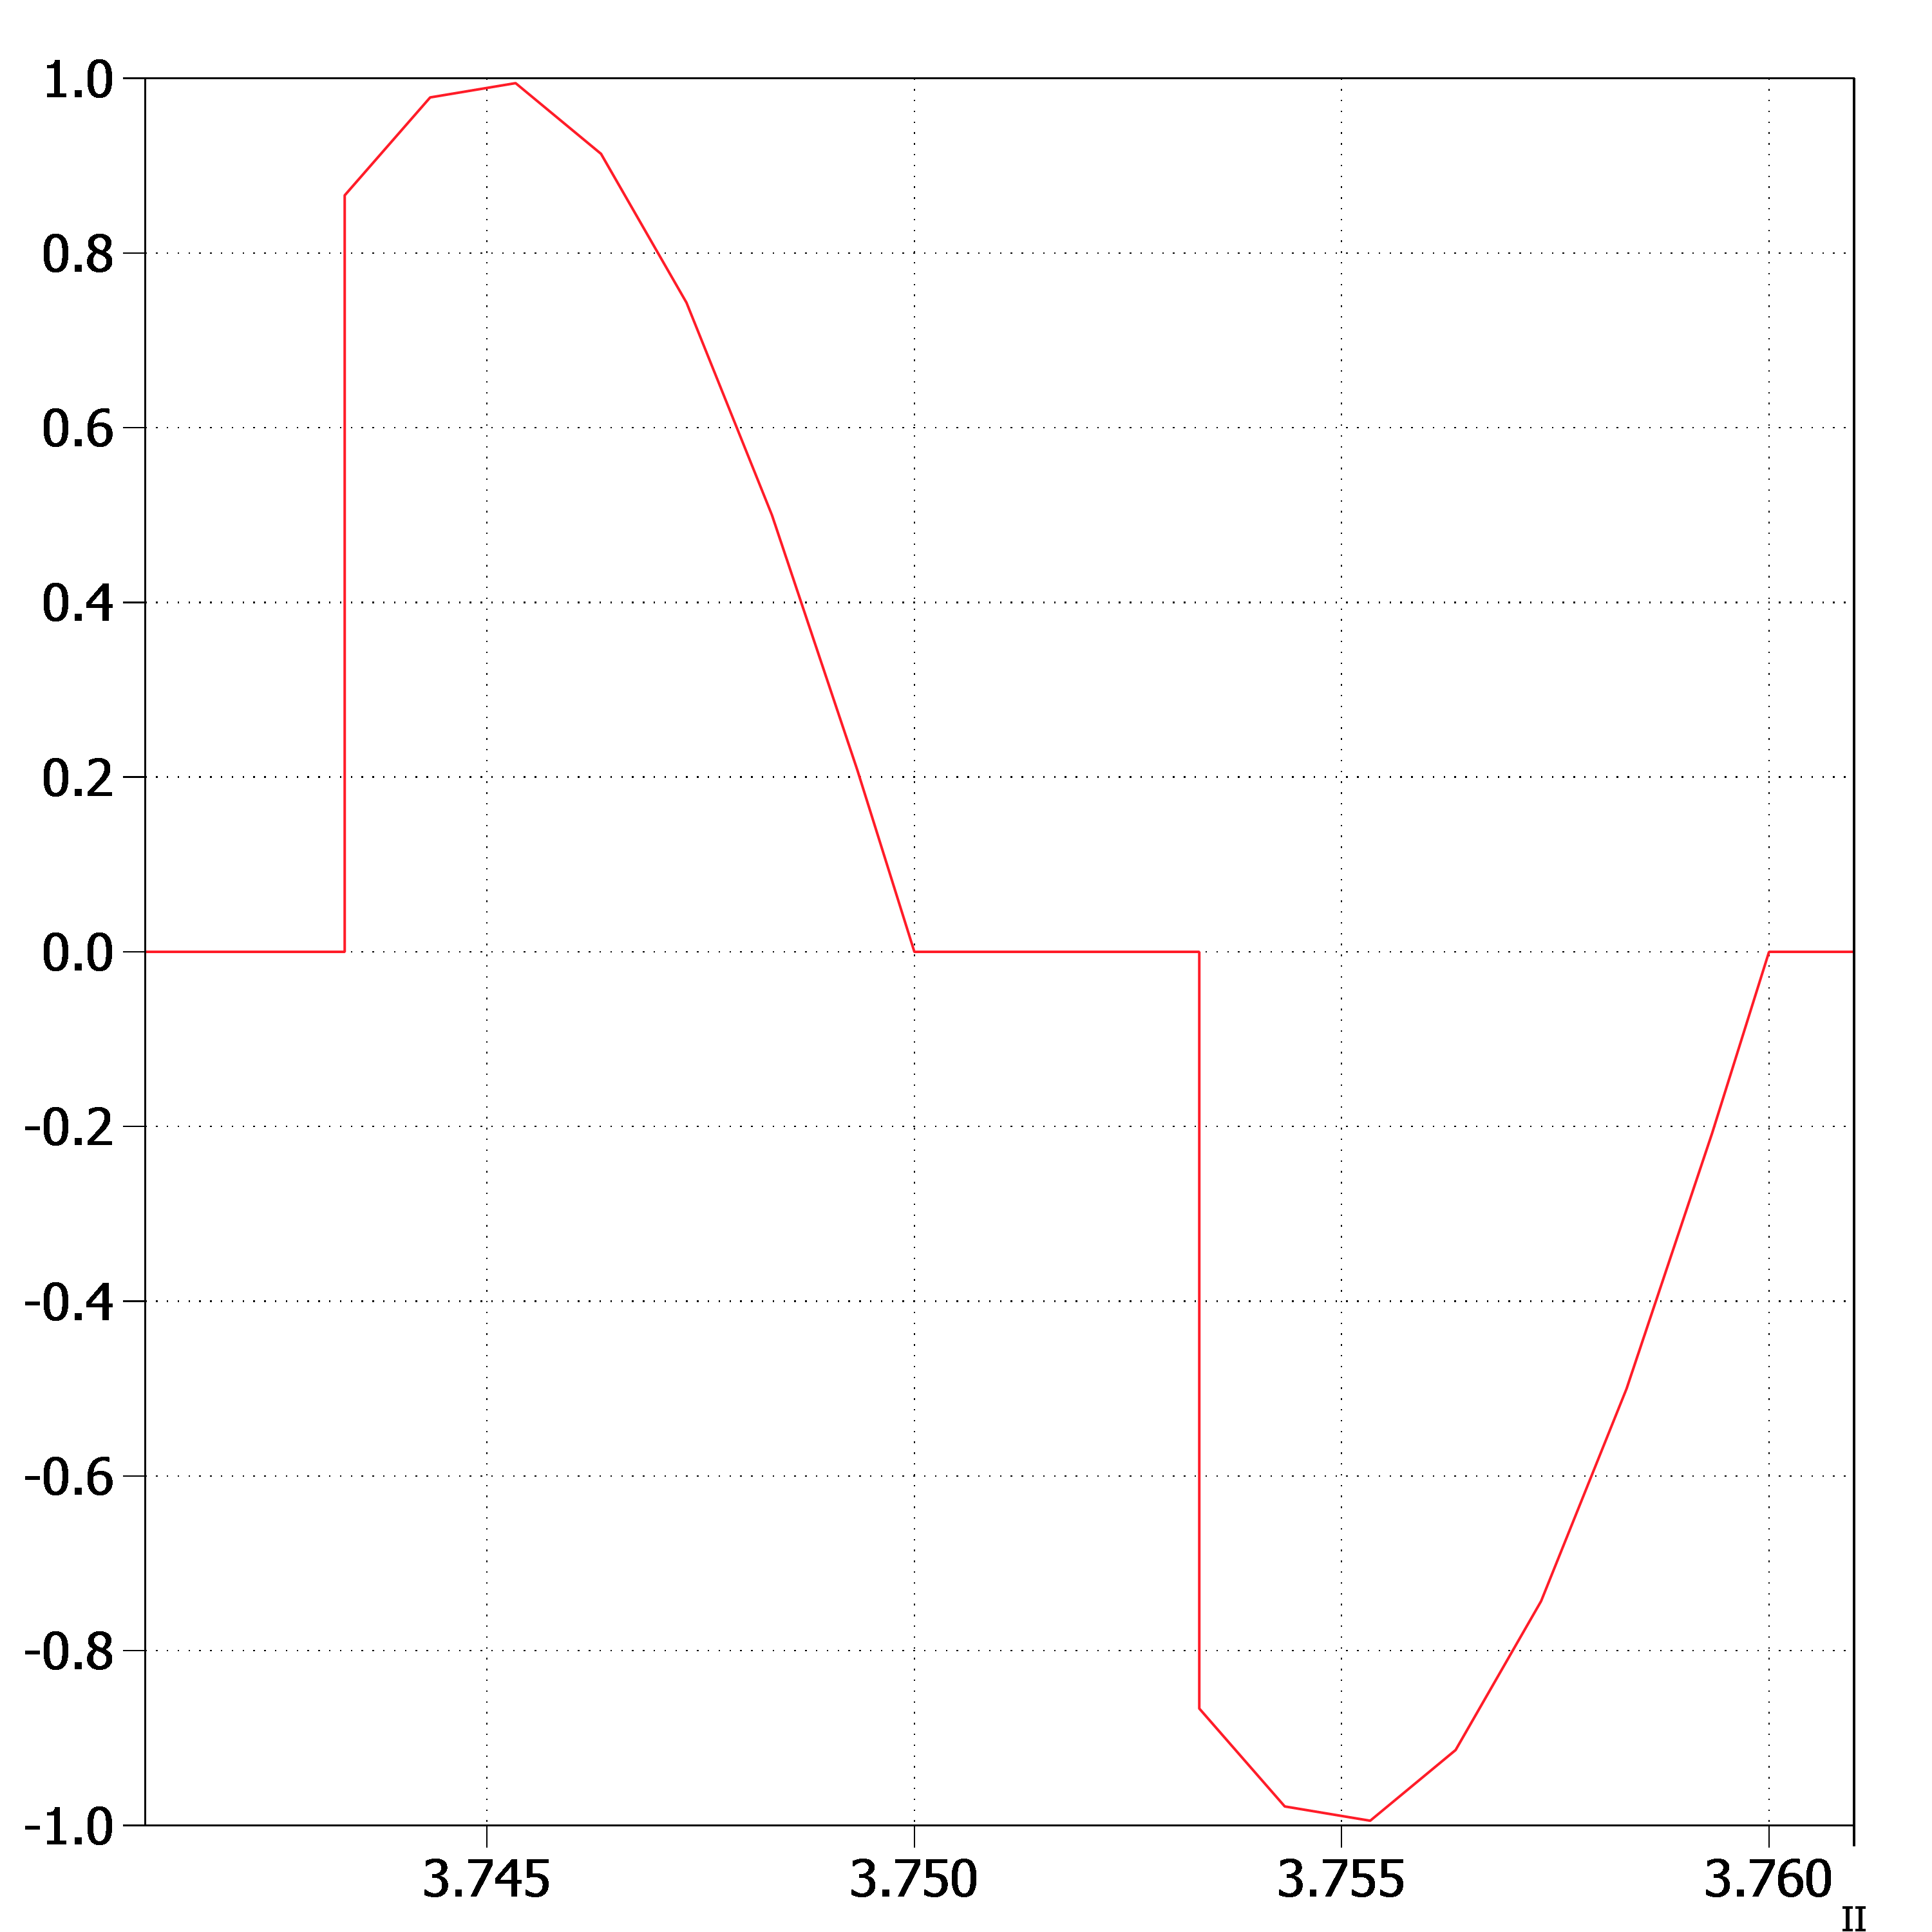
\includegraphics[width=0.43\linewidth]{plecs_phasenanschnitt_pi_3_funktion.png}\label{fig:plecs_eingangssignal_60}}\qquad
	\subfloat[][]{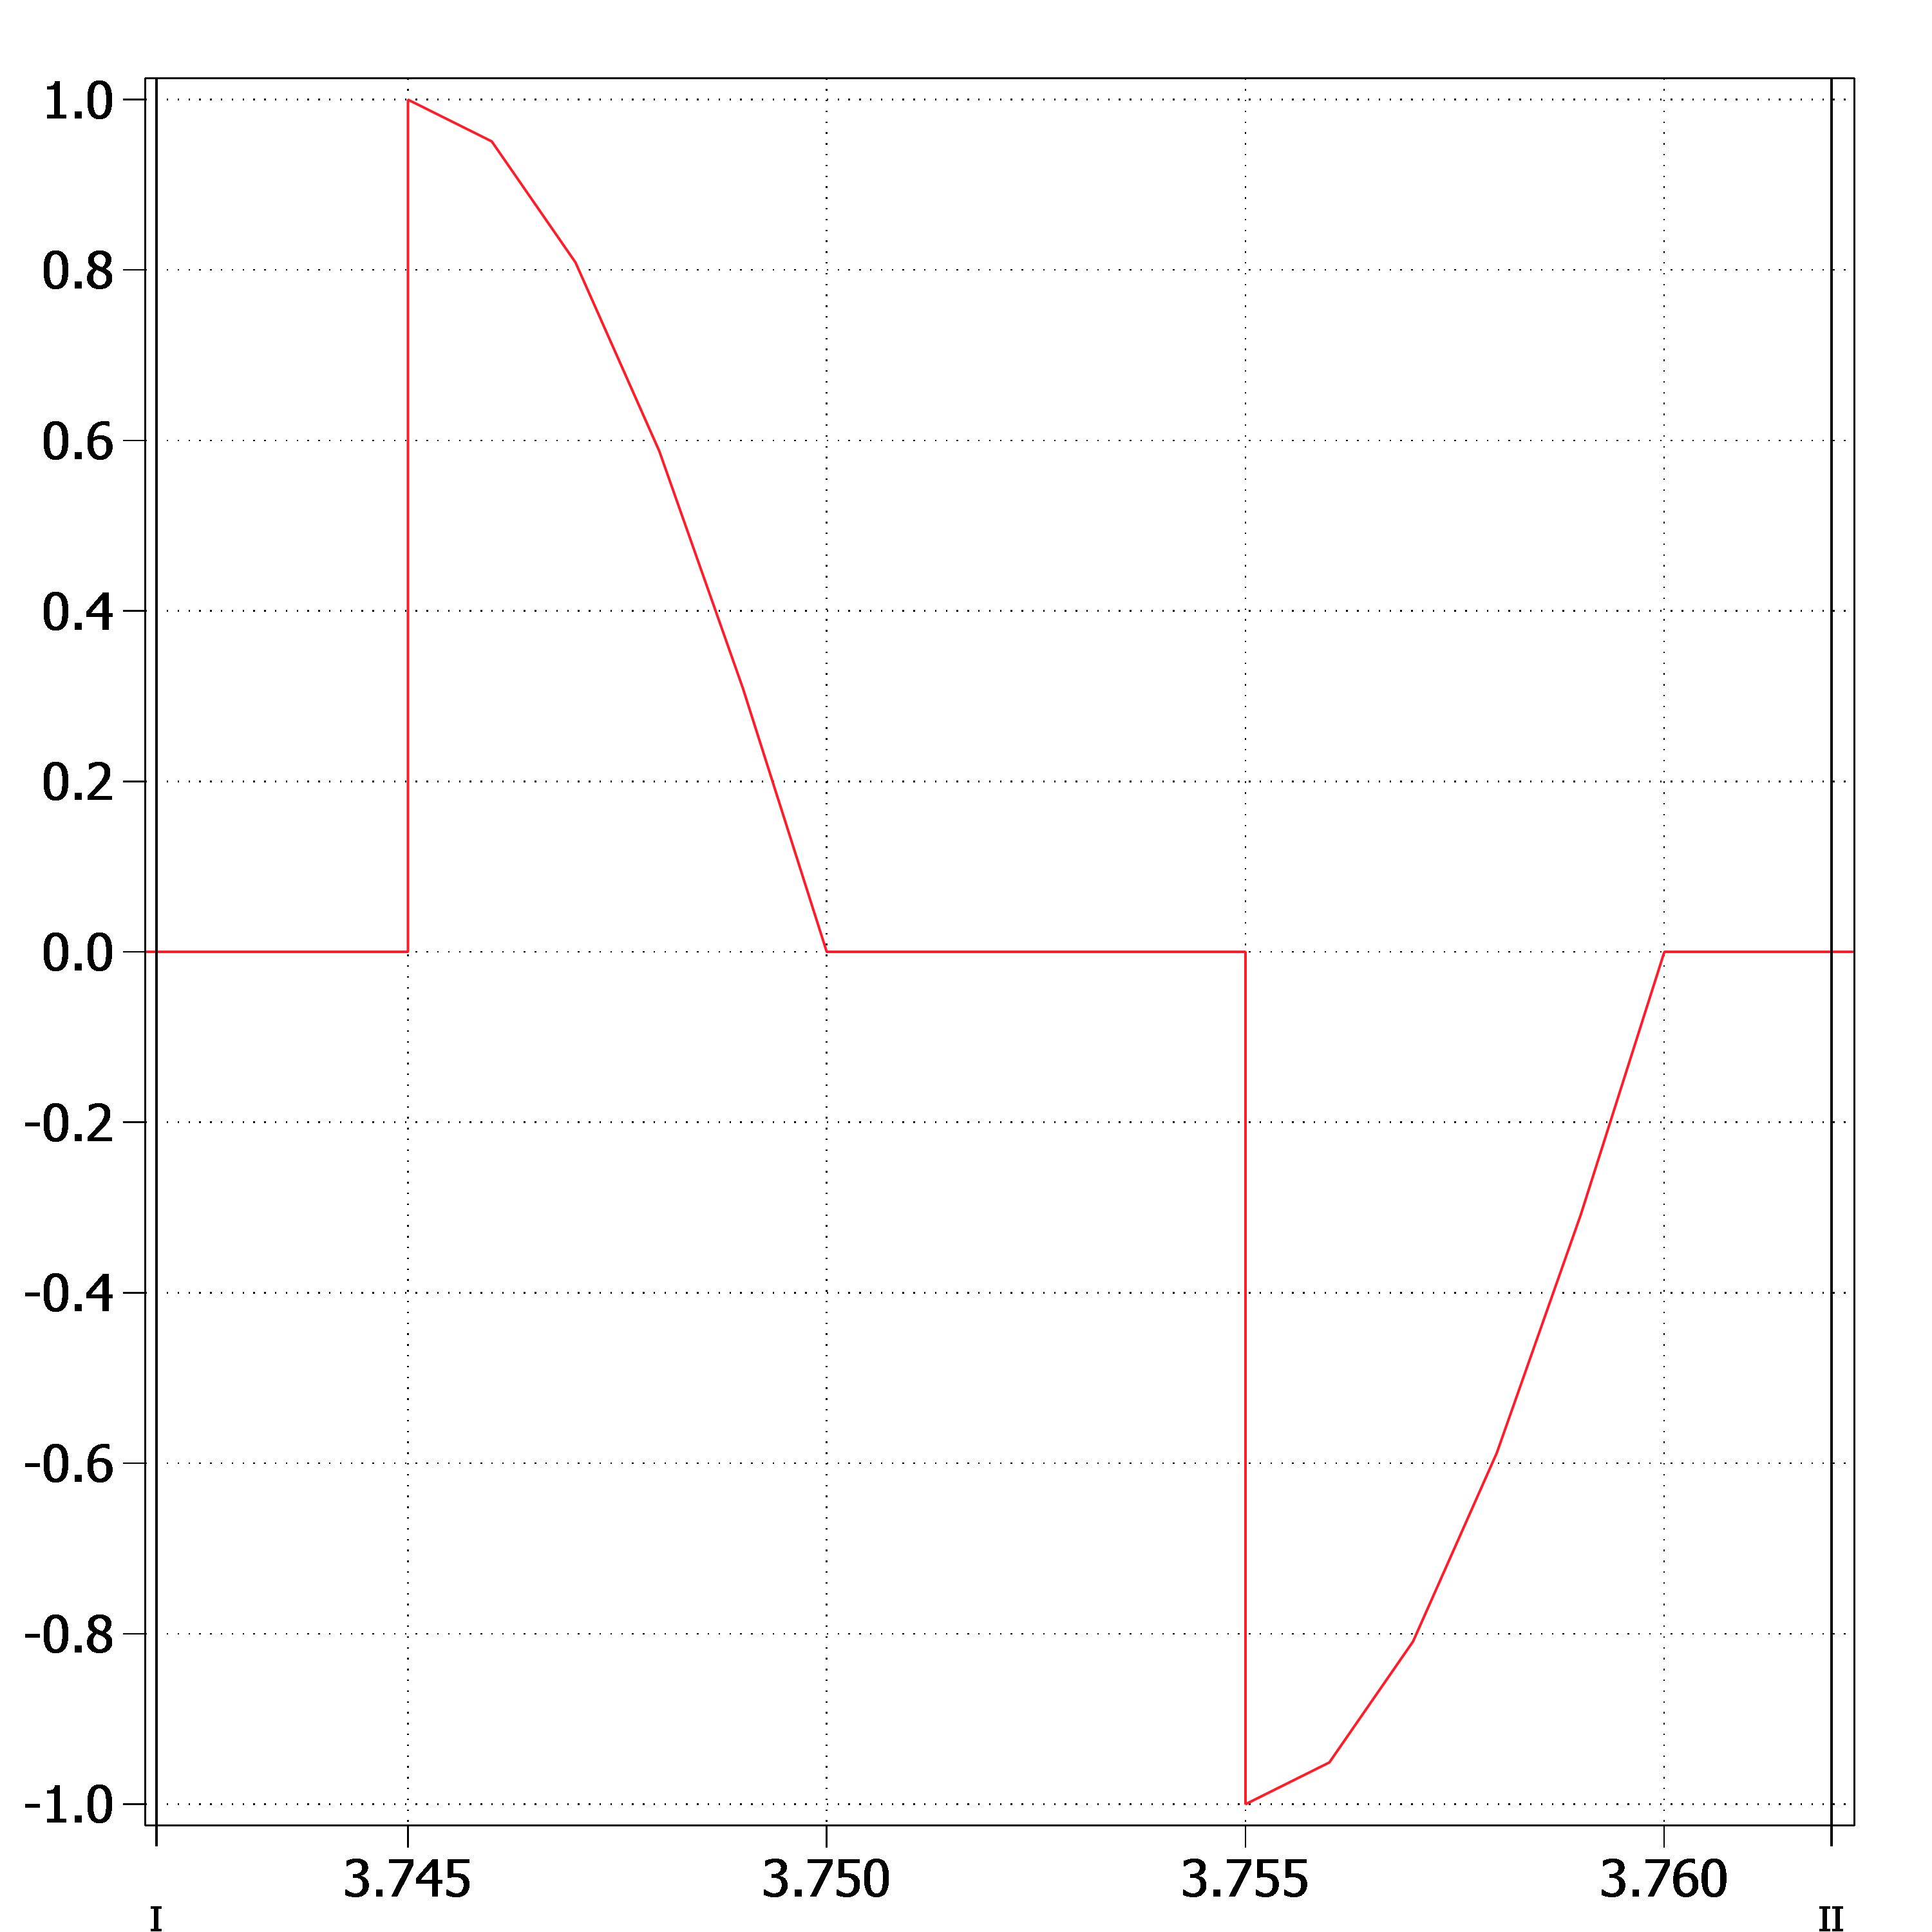
\includegraphics[width=0.43\linewidth]{plecs_phasenanschnitt_pi_2_funktion.png}\label{fig:plecs_eingangssignal_90}}
	\caption{Eingangssignal mit Phasenanschnitt (a) 60° (b) 90°}
	\label{fig:Eingangssignal simuliert mit Plecs}
\end{figure}

\newpage

Die folgenden Bilder \ref{fig:plecs_Amplitudenspektrum} zeigen das Amplitudenspektrum der Phasenanschnittsteuerung mit den zwei bereits verwendeten Winkeln. Die Grafik musst nicht wie bei der Matlab-Funktion von Hand berechnet, sondern konnte mit Hilfe des Plecs Scope direkt analysiert werden. Plecs macht auch eine Fourier-Analyse um das Spektrum anzuzeigen. Vergleicht man die Amplitudenspektren der beiden Simulationen miteinander sehen die Grafiken, nach erster Einschätzung von Auge, sehr ähnlich aus. Der genau Vergleich der Werte wird weiter unten analysiert.   
     
\begin{figure}[ht!]
	\centering
	\subfloat[][]{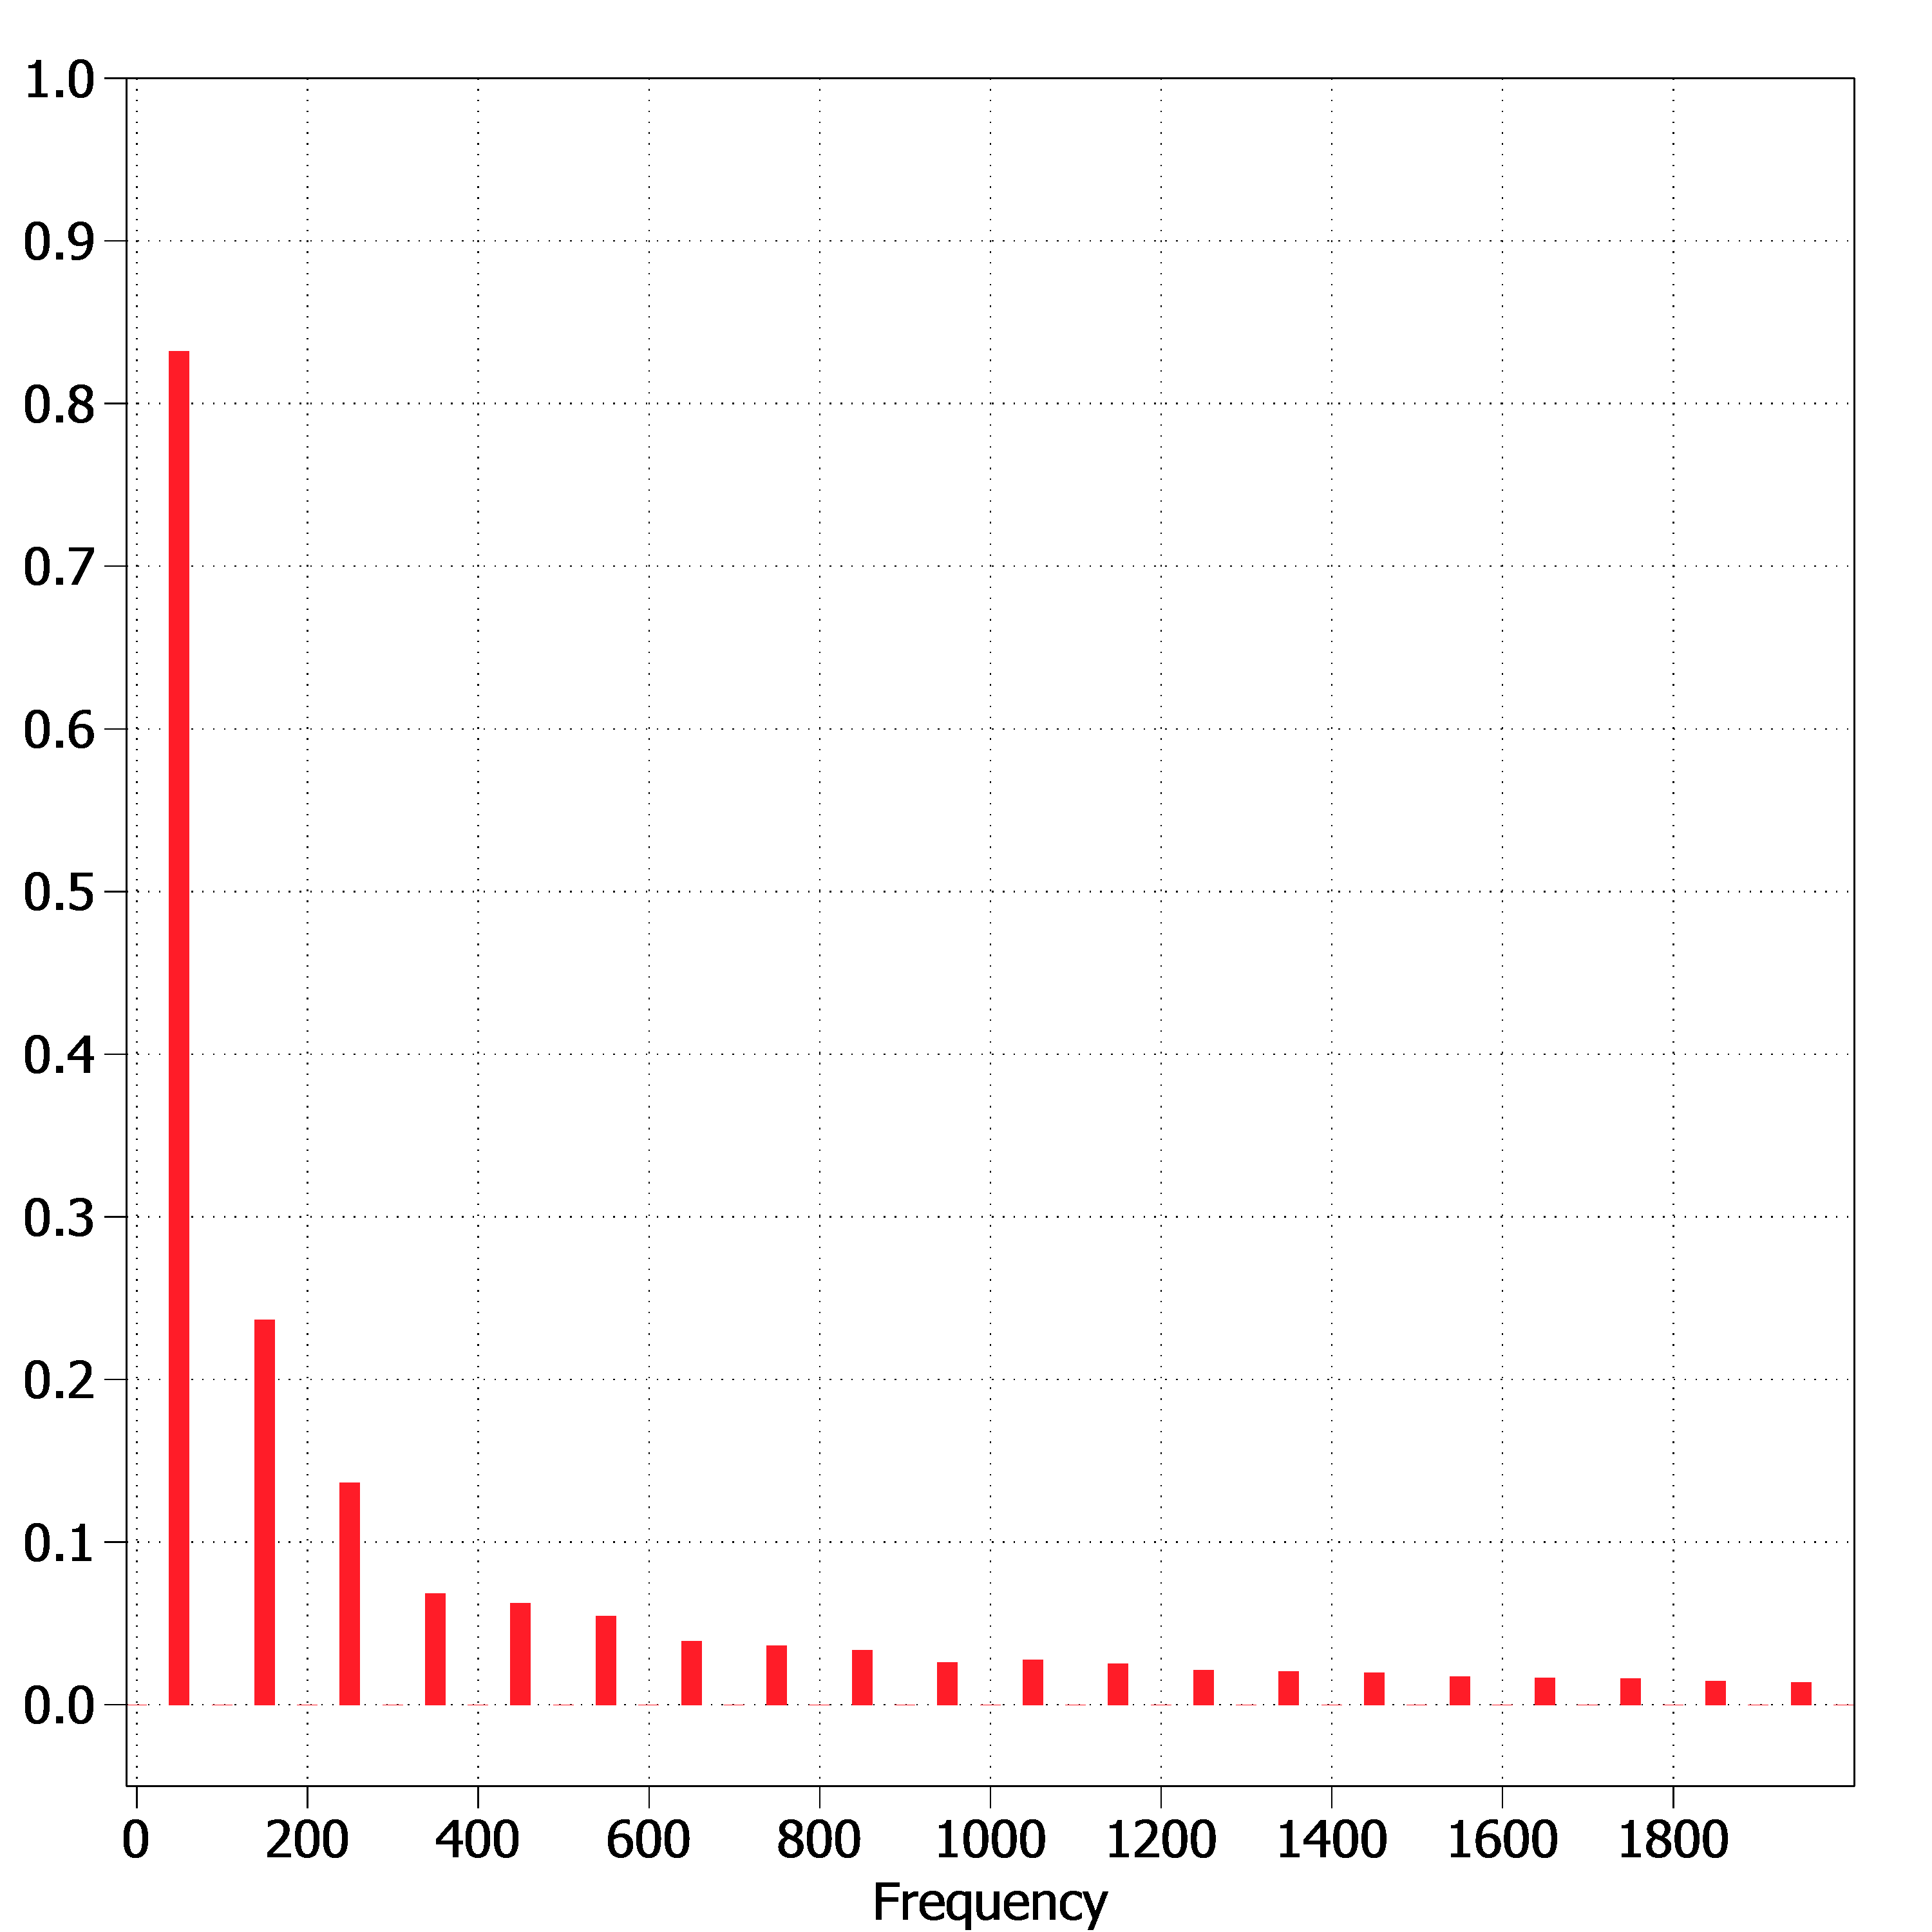
\includegraphics[width=0.43\linewidth]{plecs_phasenanschnitt_pi_3.png}\label{fig:plecs_Amplitudenspektrum_60}}\qquad
	\subfloat[][]{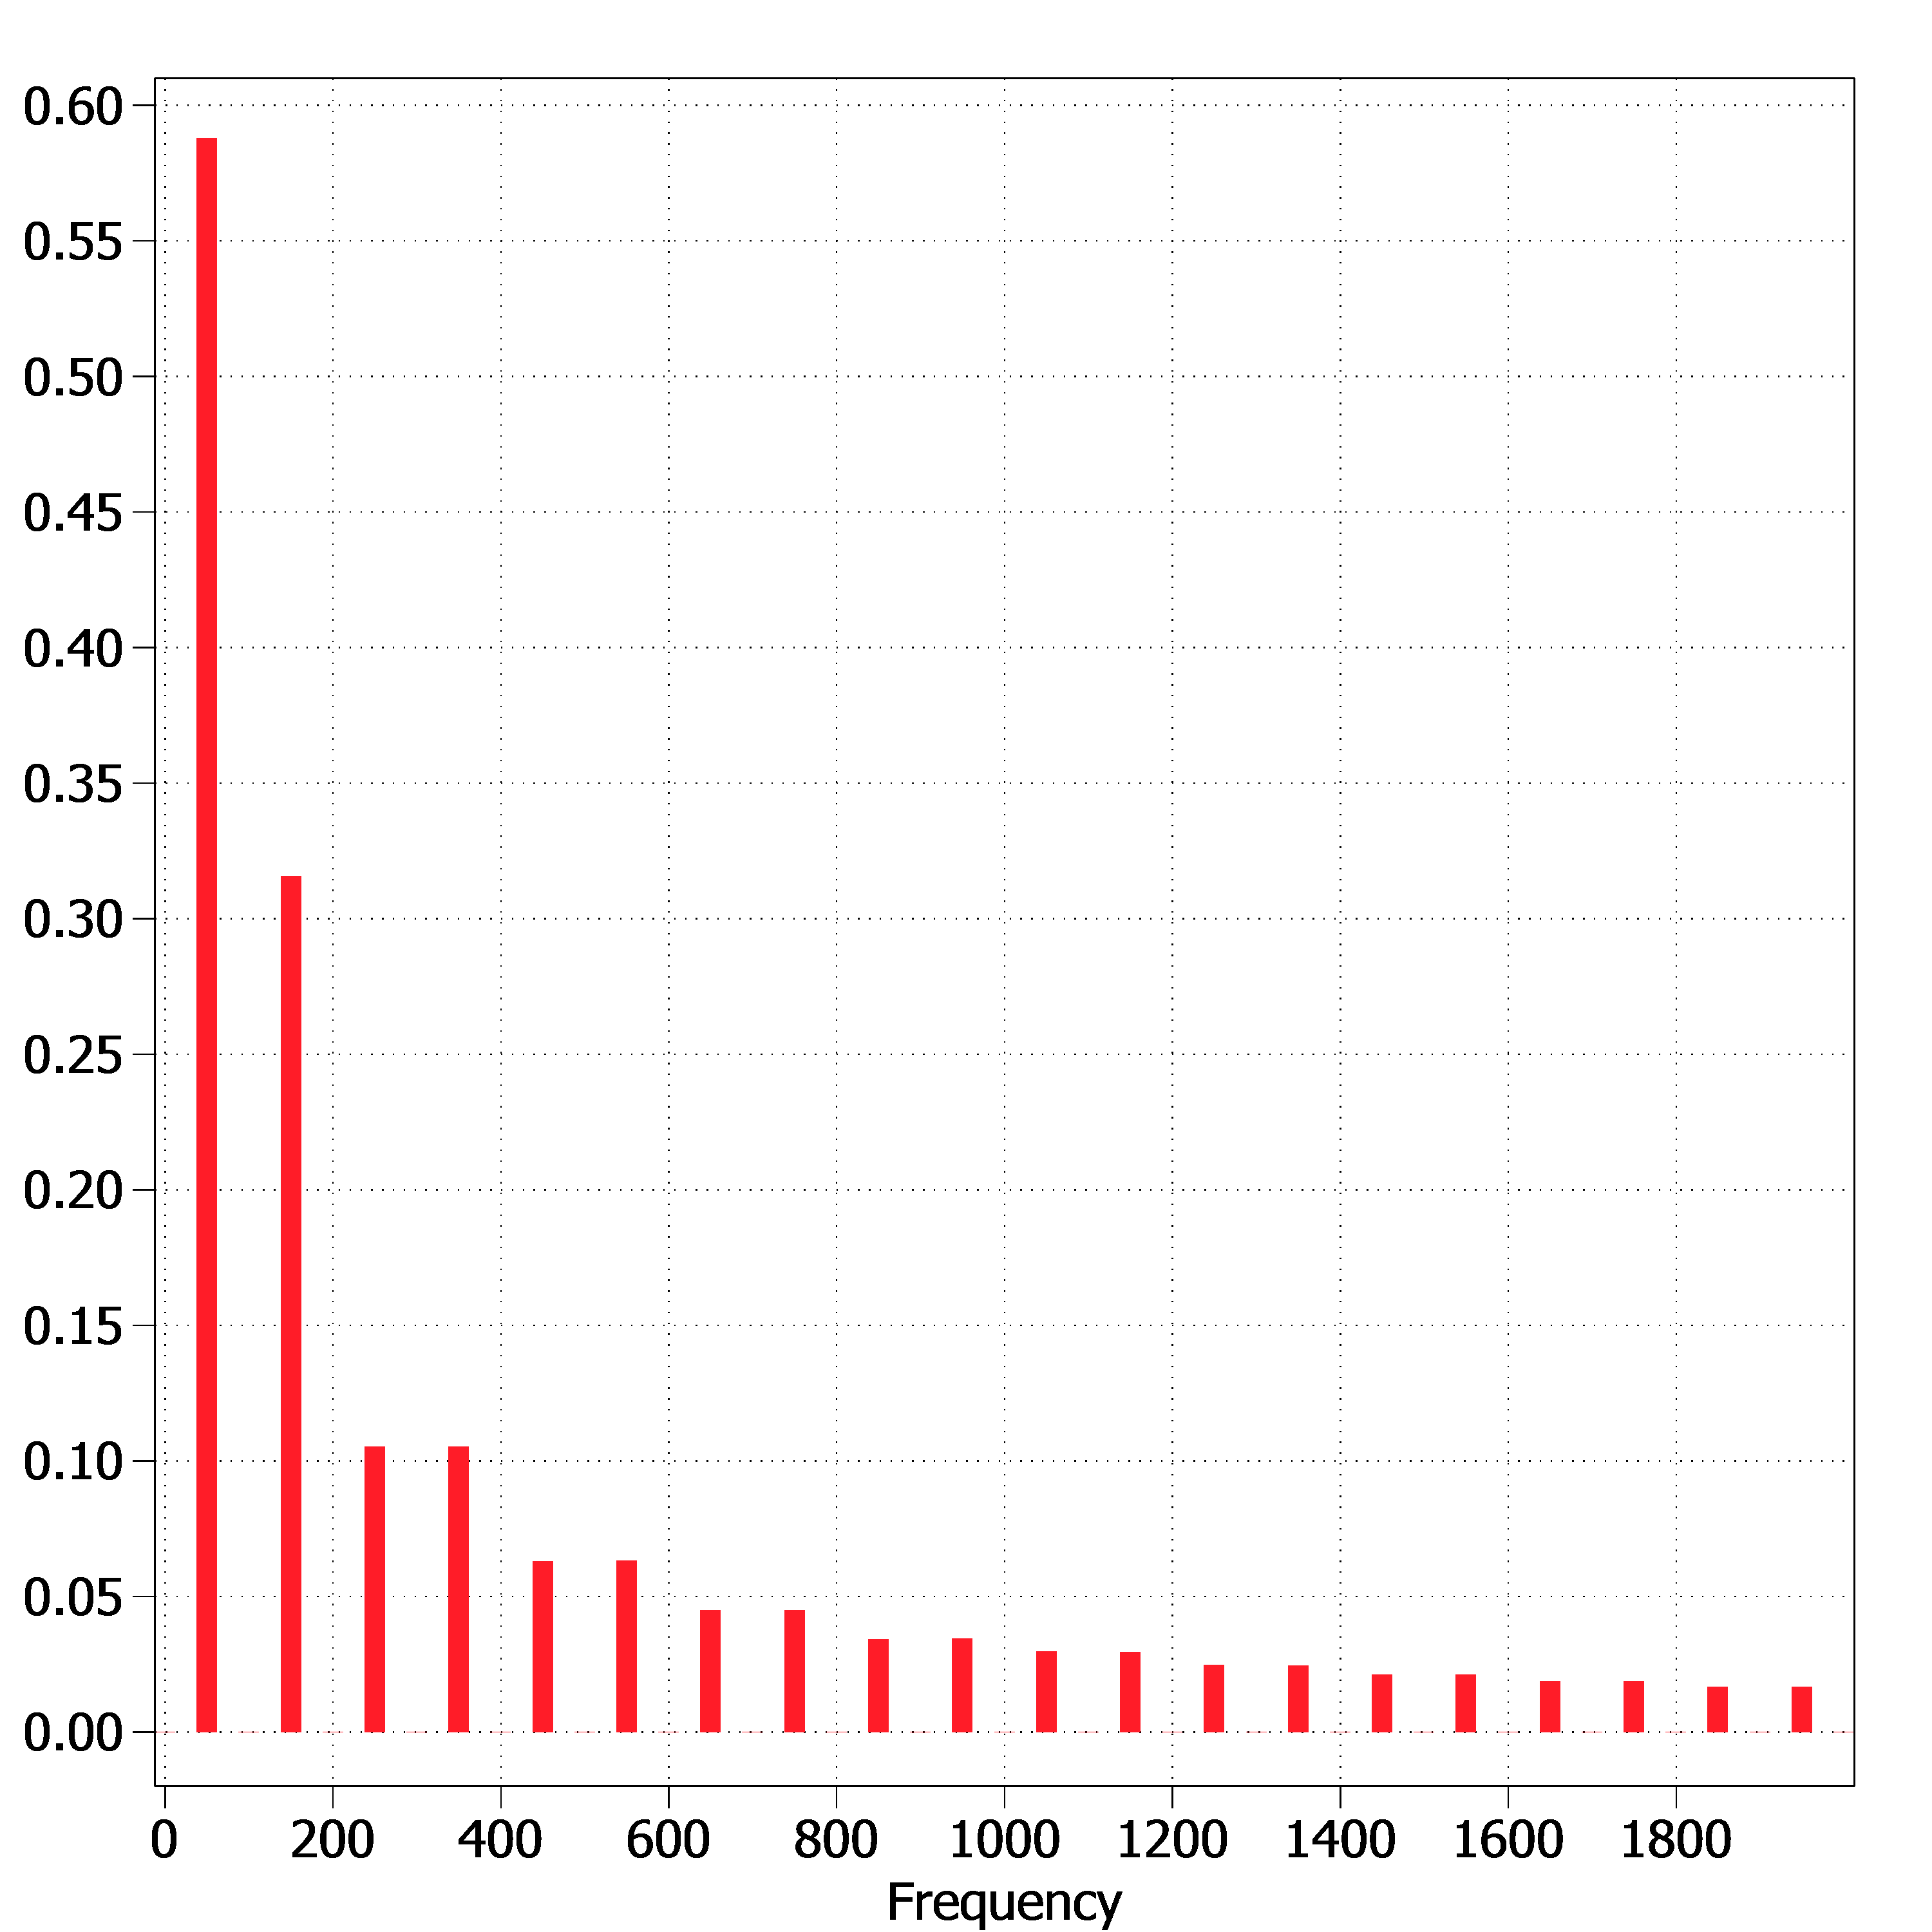
\includegraphics[width=0.43\linewidth]{plecs_phasenanschnitt_pi_2.png}\label{fig:plecs_Amplitudenspektrum_90}}
	\caption{Amplitudenspektrum (a) 60° (b) 90°}
	\label{fig:plecs_Amplitudenspektrum}
\end{figure}

Als nächstes wurde eine Simulation für die Schwingungspaketsteuerung aufgebaut \ref{fig:plecs_Schwingungspakete}. Auch hier verwendete man einen duty cycle von 0.5 in Bild  \ref{fig:plecs_Schwingungspaket_0_5} beziehungsweise 0.8 in der Darstellung \ref{fig:plecs_Schwingungspaket_0_8}.  
\begin{figure}[ht!]
	\centering
	\subfloat[][]{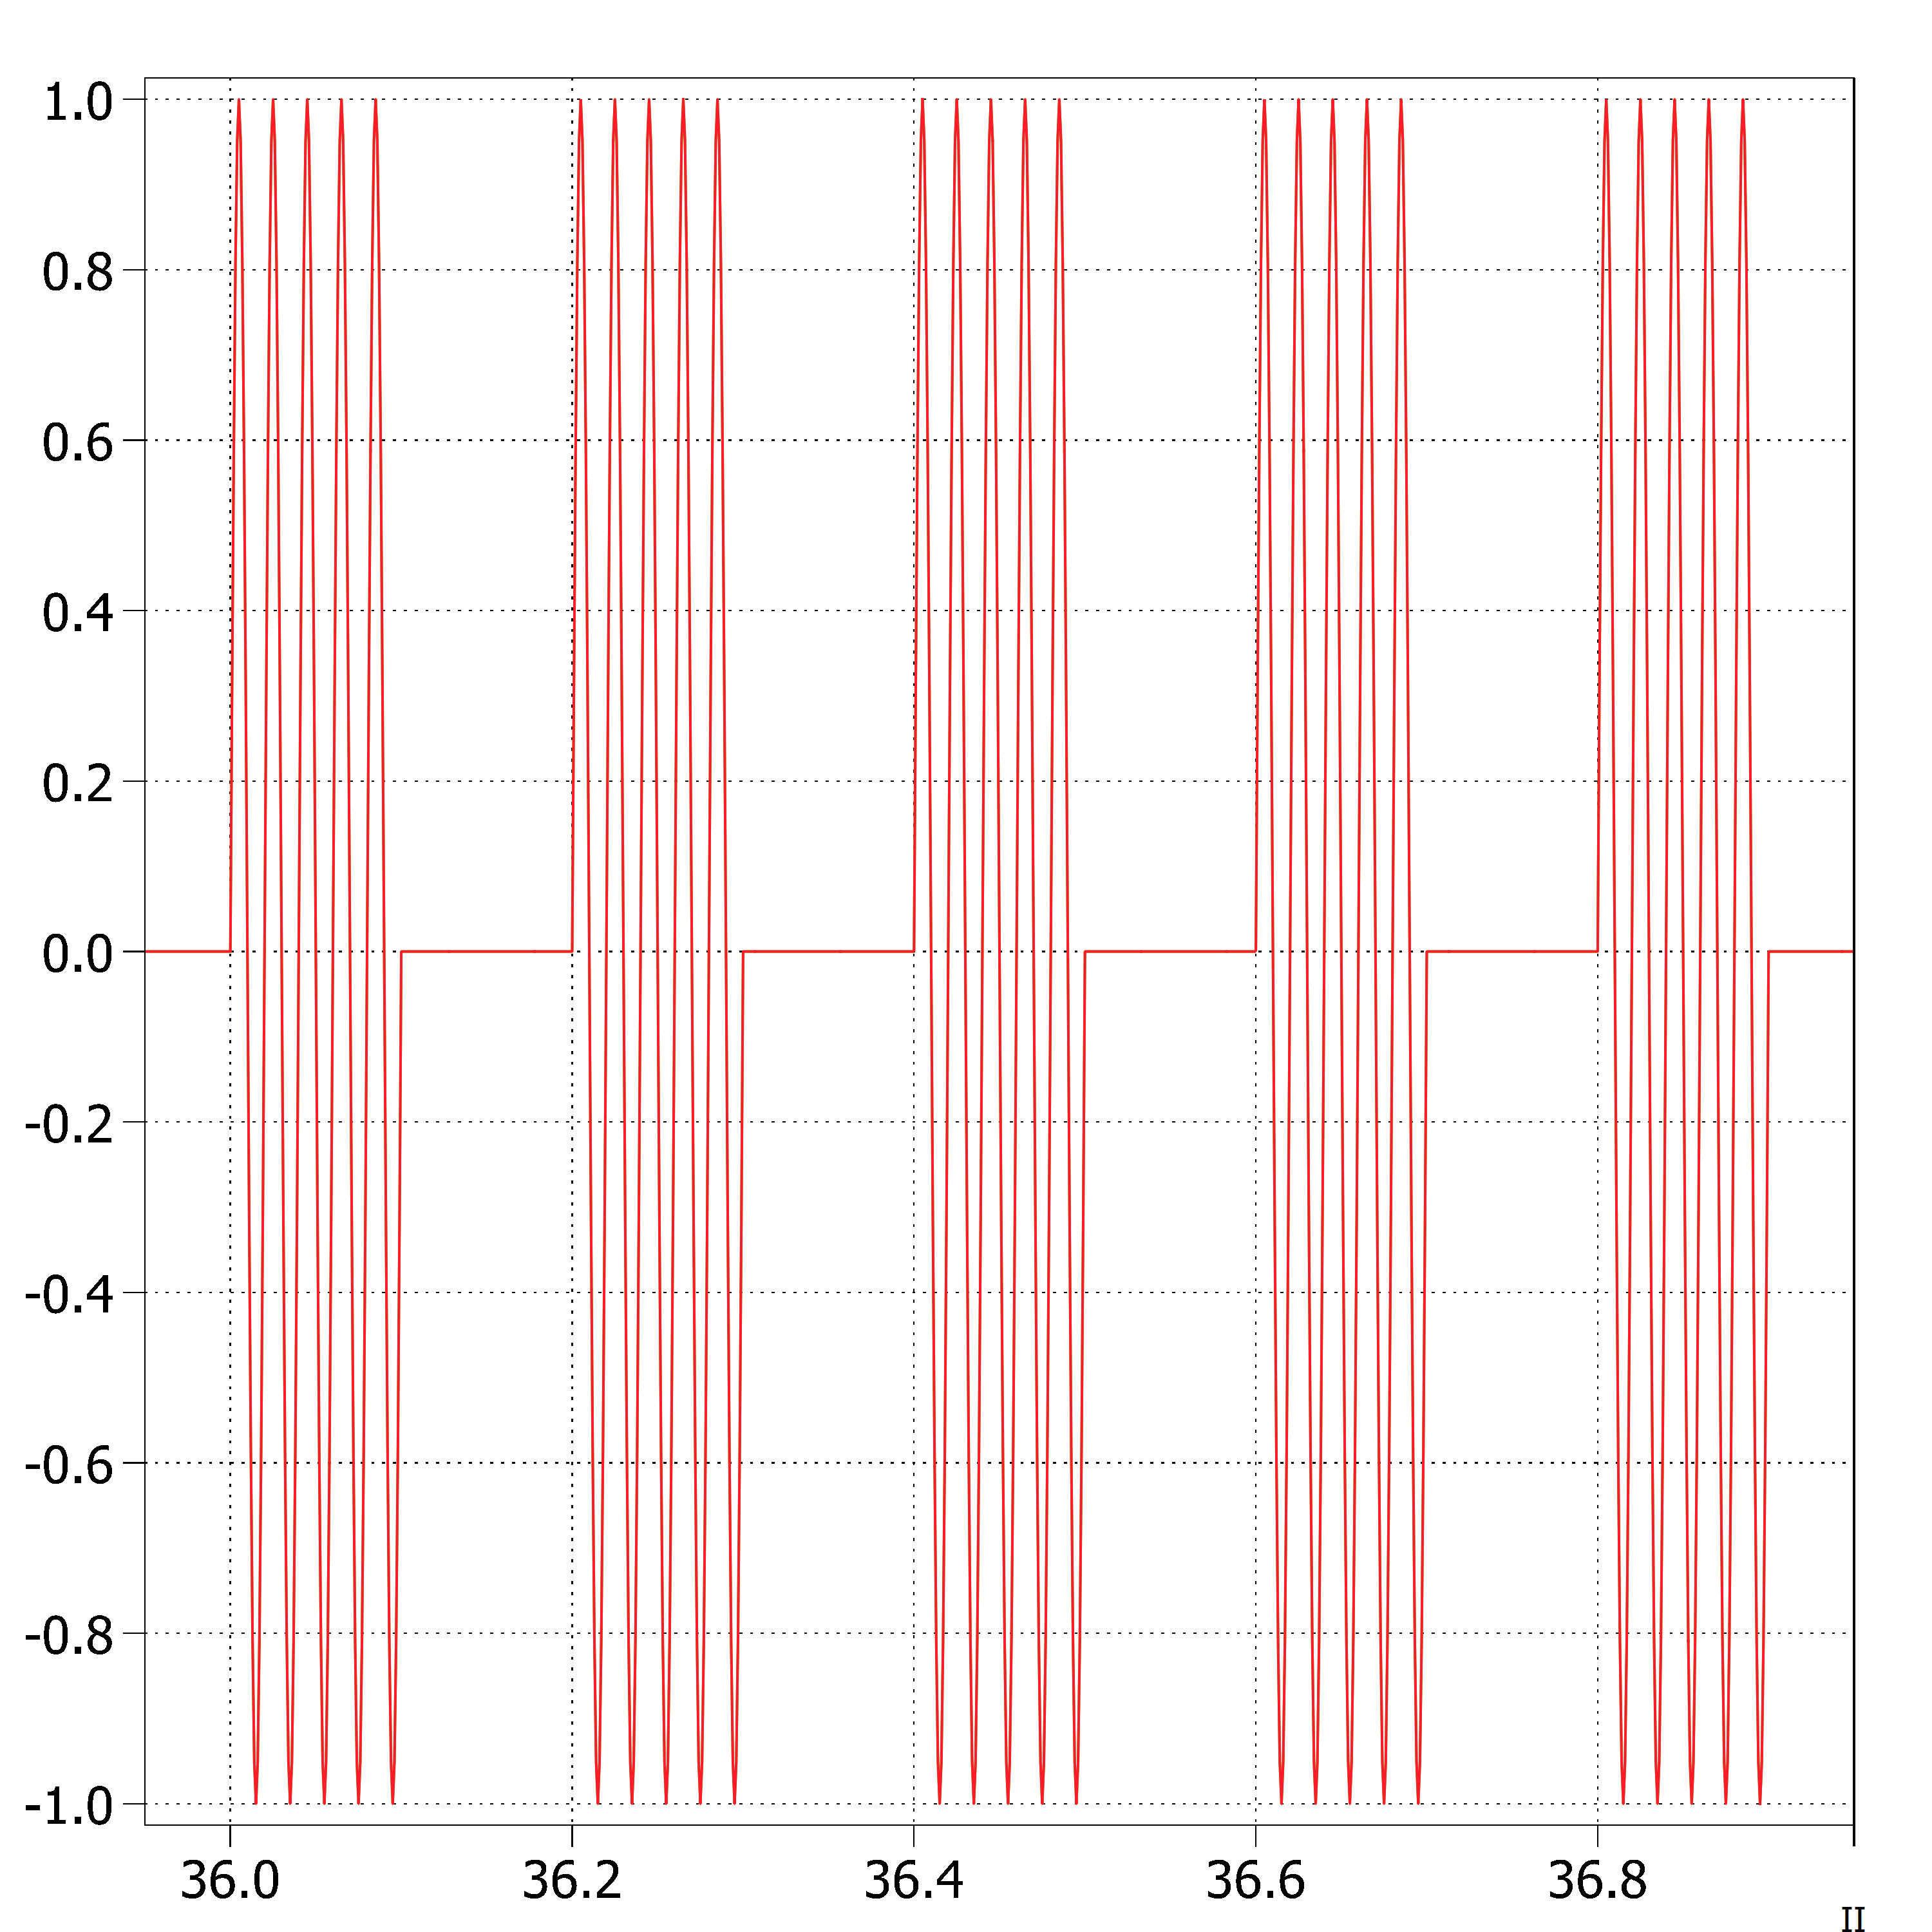
\includegraphics[width=0.45\linewidth]{plecs_schwingungspacket_0_5_schwingungen.PNG}\label{fig:plecs_Schwingungspaket_0_5}}\qquad
	\subfloat[][]{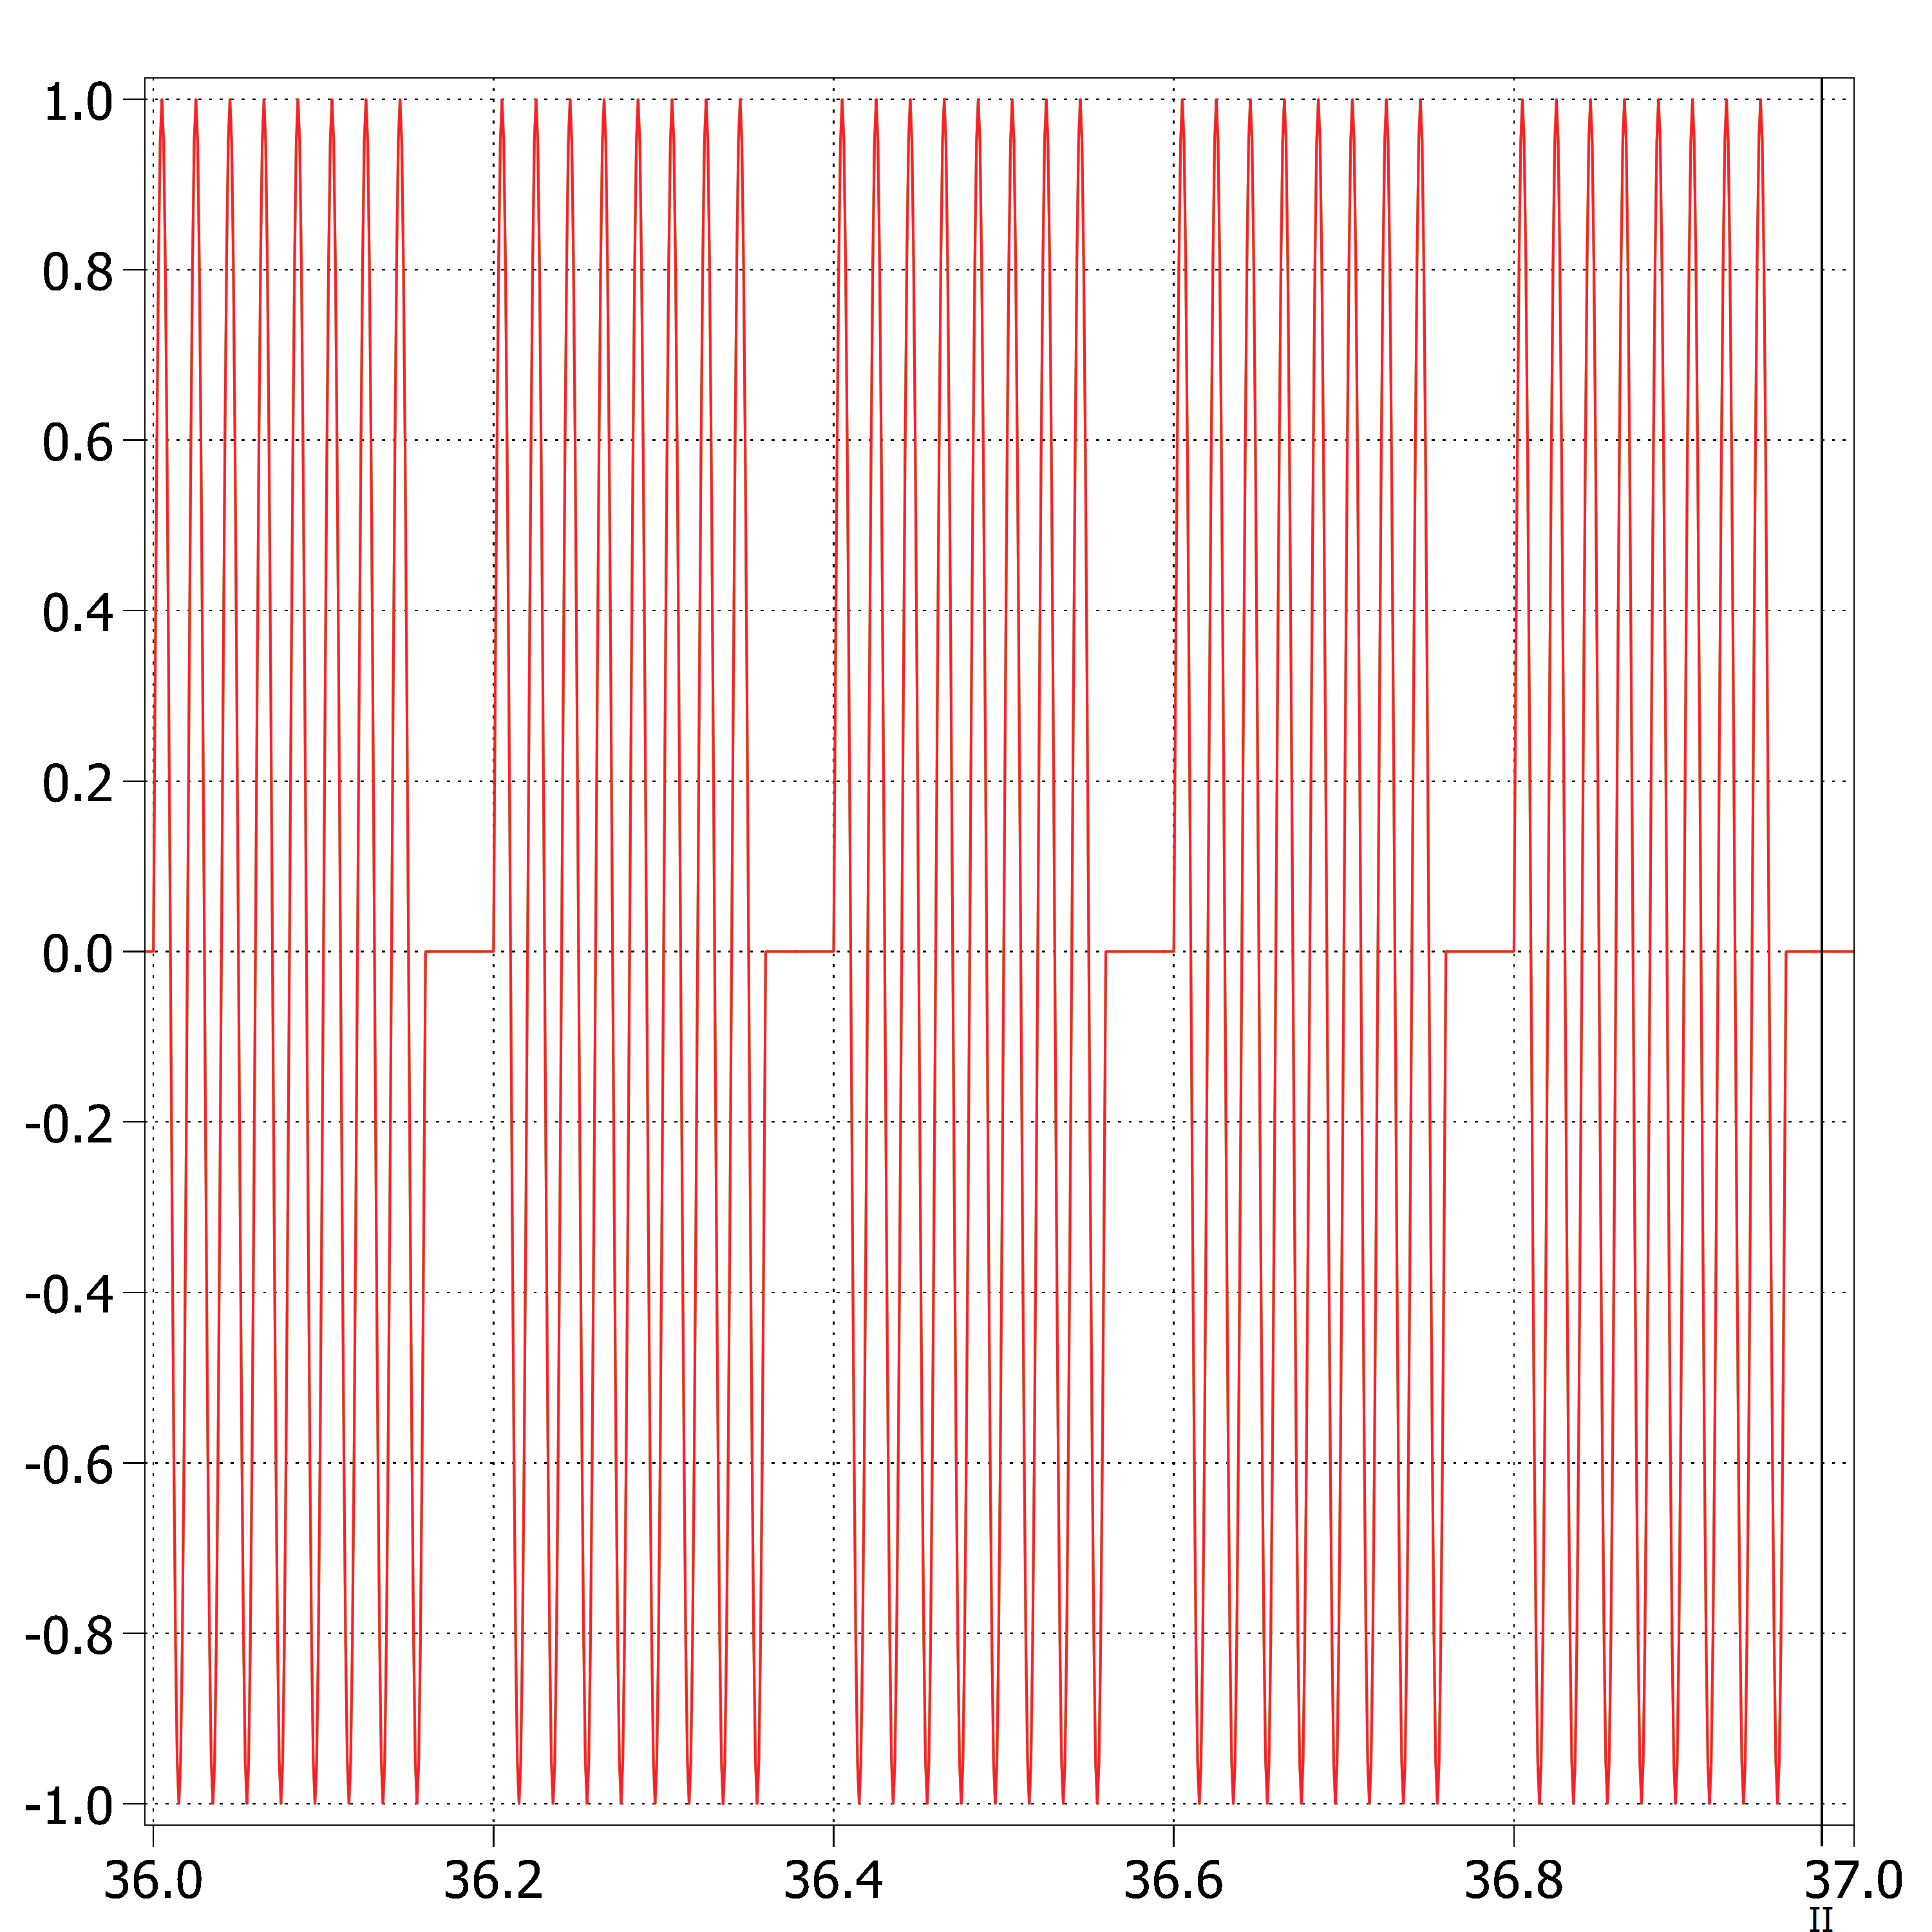
\includegraphics[width=0.45\linewidth]{plecs_schwingungspacket_0_8_schwingungen.PNG}\label{fig:plecs_Schwingungspaket_0_8}}
	\caption{Schwingungspaket mit einem duty cycle (a) 0.5 (b) 0.8}
	\label{fig:plecs_Schwingungspakete}
\end{figure}

In der folgende Abbildung \ref{fig:plecs_Schwingungspakete_Amplitudenspektrum_ 0_5_100_1000} wurde das Amplitudenspektrum des Schwingungspaketes mit einem duty cycle von 0.5 dargestellt. Auf der linken Seite der Abbildung \ref{fig:plecs_Schwingungspaket_0_5_100} erkennt man das bekannte Spektrum von 0- 100 Hz mit den Subharmonischen Werten unterhalb von 50 Hz und den Zwischenharmonischen Schwingungen von 50 Hz -100 Hz. In der rechten Grafik  \ref{fig:plecs_Schwingungspaket_0_5_1000} erweiterte man das Spektrum bis zu 1000 Hz. Auch hier ist eine optische Ähnlichkeit zur  Matlab-Funktion ersichtlich.     
\begin{figure}[ht!]
	\centering
	\subfloat[][]{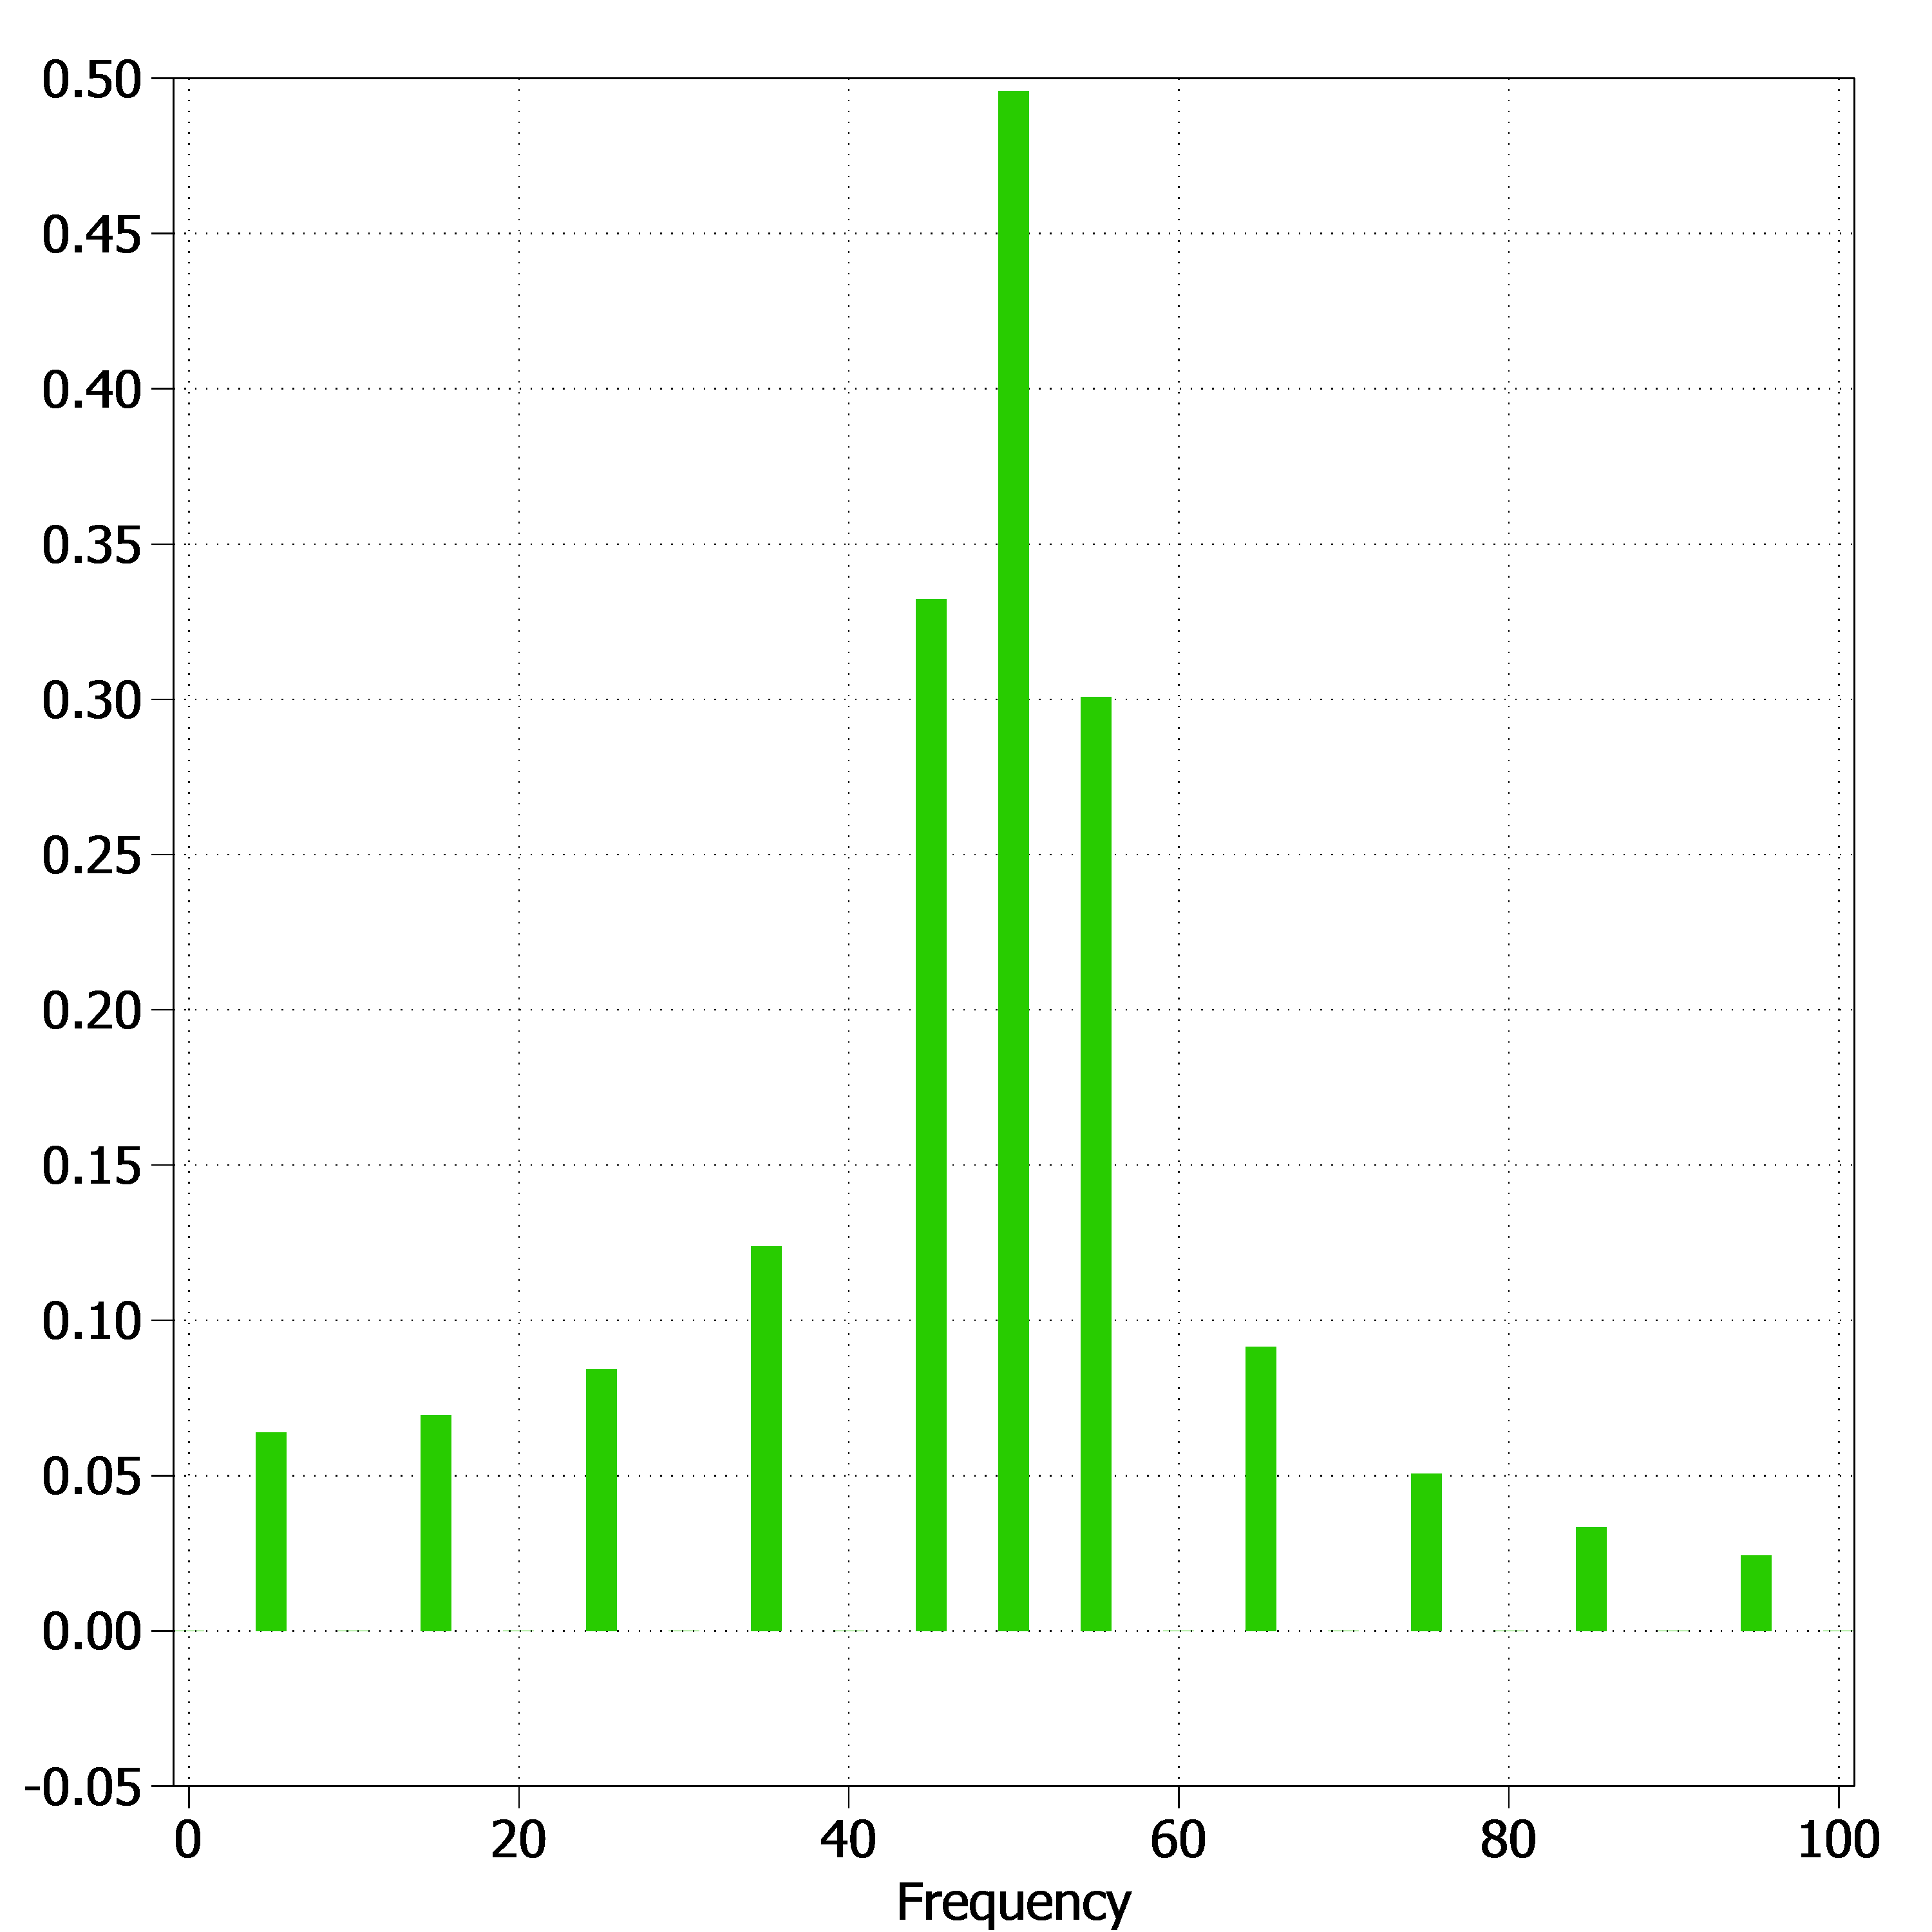
\includegraphics[width=0.45\linewidth]{plecs_schwingungspacket_0_5_100.PNG}\label{fig:plecs_Schwingungspaket_0_5_100}}\qquad
	\subfloat[][]{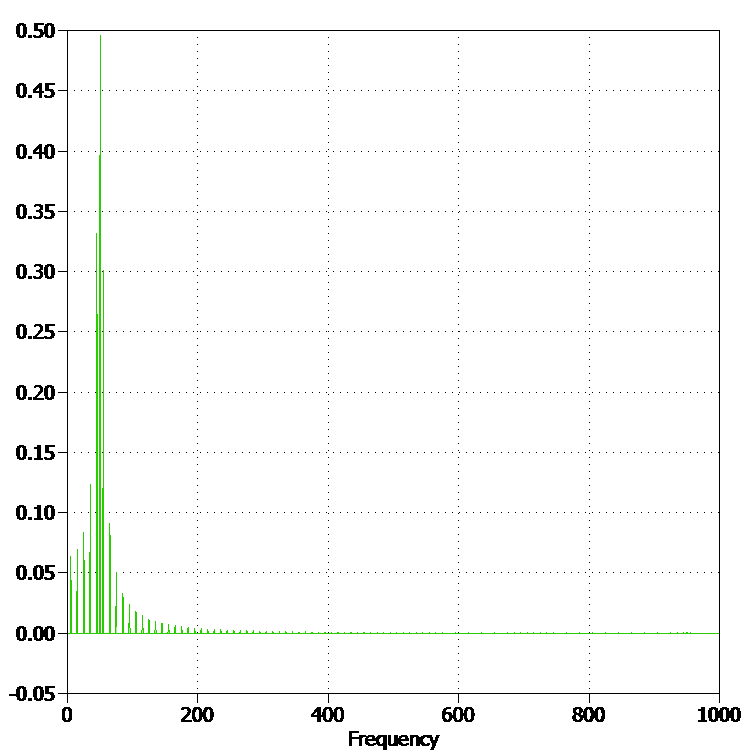
\includegraphics[width=0.45\linewidth]{plecs_schwingungspacket_0_5_1000.PNG}\label{fig:plecs_Schwingungspaket_0_5_1000}}
	\caption{Amplitudenspektrum mit einem duty cycle 0.5 von (a) 0 - 100 Hz (b) 0 - 1000 Hz}
	\label{fig:plecs_Schwingungspakete_Amplitudenspektrum_ 0_5_100_1000}
\end{figure}


Vollständigkeits halber realisierte man das gleiche noch mit einem duty cycle von 0.8. Auch hier ist das Spektrum, in der linken Abbildung \ref{fig:plecs_Schwingungspaket_0_8_100} mit einer Frequenz von 0 - 100 Hz und im rechten Bild \ref{fig:plecs_Schwingungspaket_0_8_1000} bis 1000 Hz, dargestellt. 


\begin{figure}[ht!]
	\centering
	\subfloat[][]{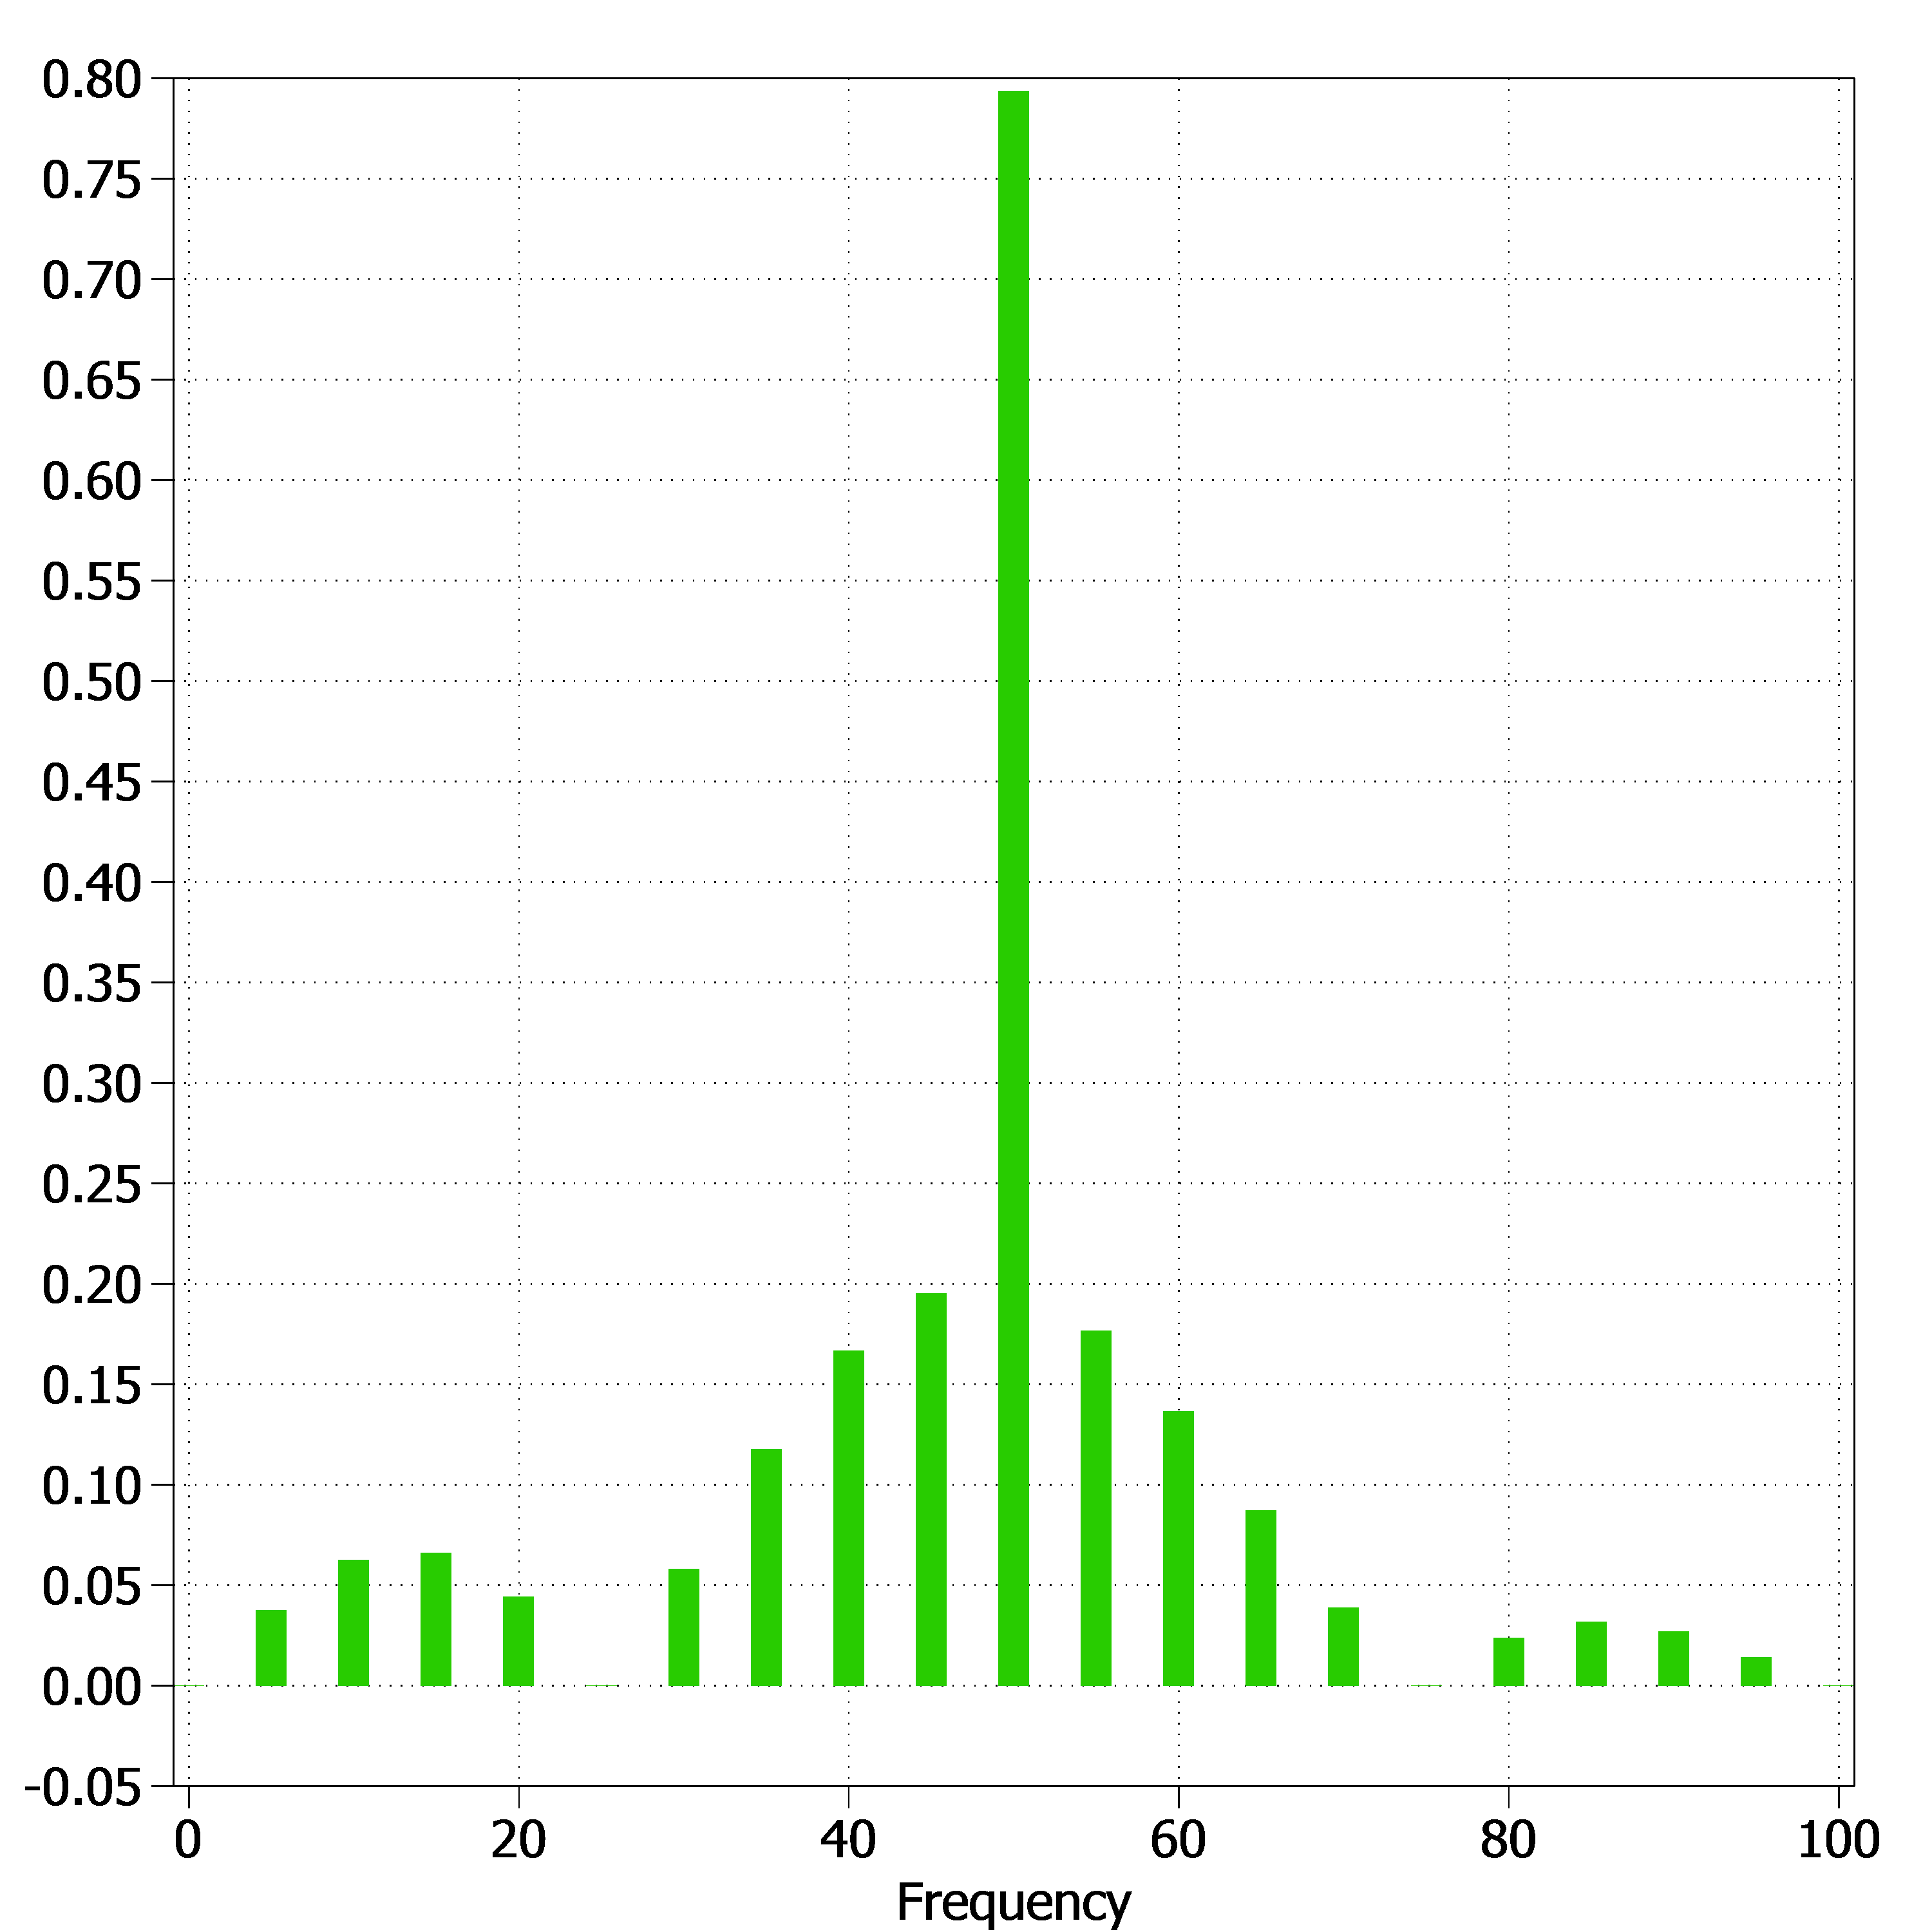
\includegraphics[width=0.45\linewidth]{plecs_schwingungspacket_0_8.PNG}\label{fig:plecs_Schwingungspaket_0_8_100}}\qquad
	\subfloat[][]{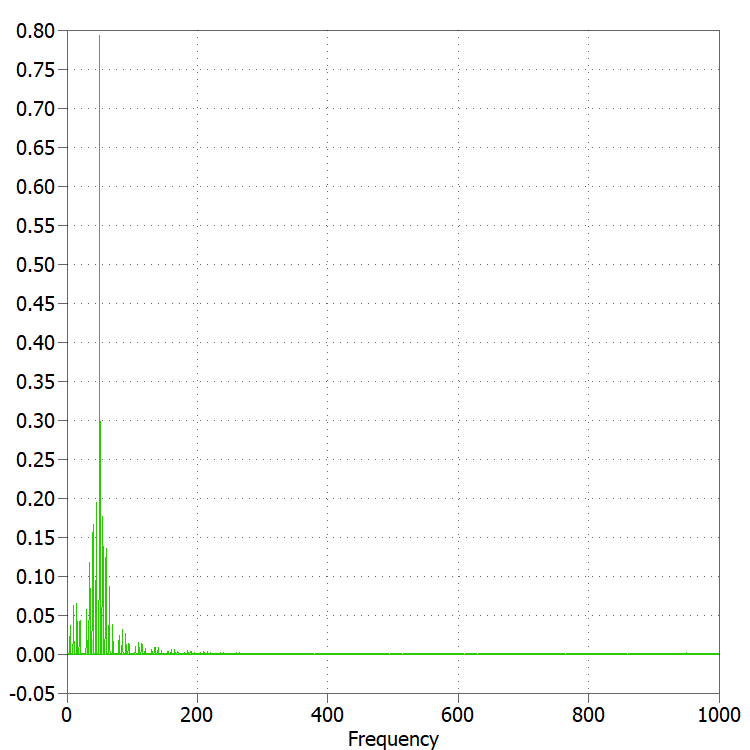
\includegraphics[width=0.45\linewidth]{plecs_schwingungspacket_0_8_1000.PNG}\label{fig:plecs_Schwingungspaket_0_8_1000}}
	\caption{Amplitudenspektrum mit einem duty cycle 0.8 von (a) 0 - 100 Hz (b) 0 - 1000 Hz}
	\label{fig:plecs_Schwingungspakete_Amplitudenspektrum_ 0_8_100_1000}
\end{figure}


Letztlich wurde noch das lineare absolute Spektrum der beiden duty cyclen, 0.5 in Bild \ref{fig:plecs_Schwingungspaket_0_5_absolut_log} und 0.8 in Abbildung \ref{fig:plecs_Schwingungspaket_0_8_absolut_log}, veranschaulicht. Damit man die Grafiken mit der Matlab-Simulation vergleichen konnte, entschied man sich das Spektrum bis zu einer Frequenz von 100 Hz anzuzeigen. Auch hier erkennt man eine optische Ähnlichkeit zur Matlab-Simulation. 


\begin{figure}[ht!]
	\centering
	\subfloat[][]{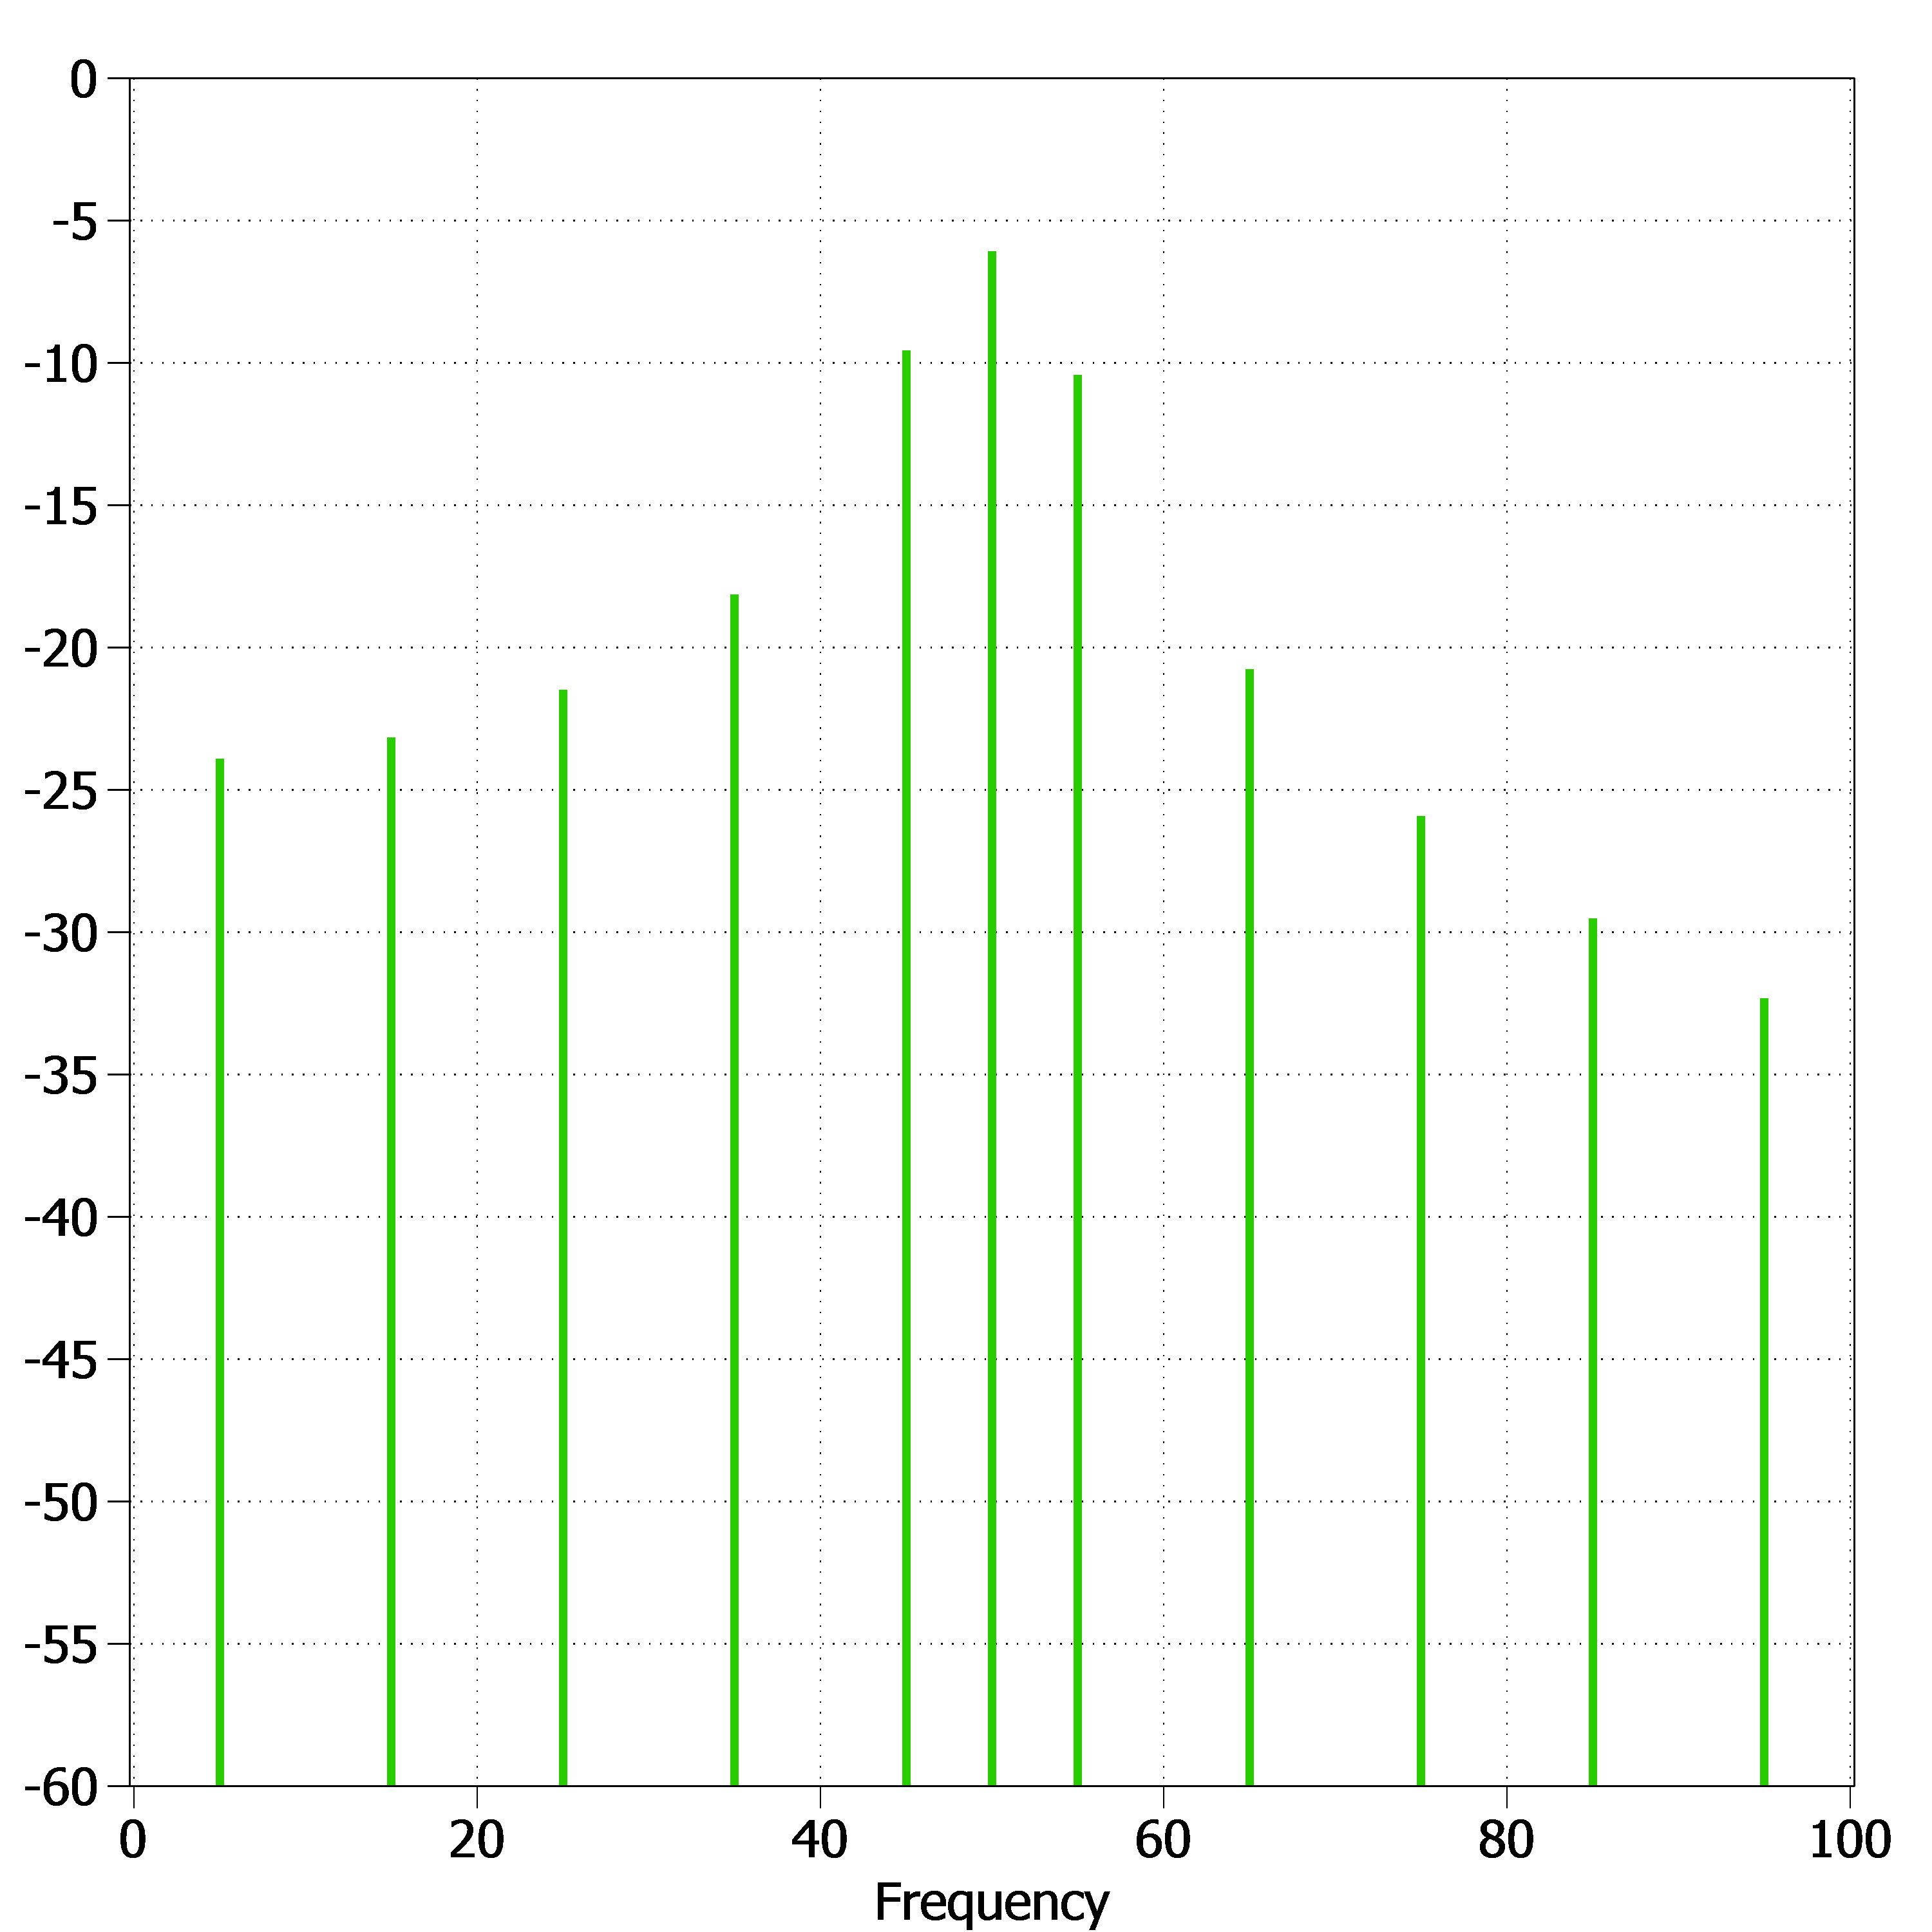
\includegraphics[width=0.45\linewidth]{plecs_schwingungspacket_0_5_absolut_log.PNG}\label{fig:plecs_Schwingungspaket_0_5_absolut_log}}\qquad
	\subfloat[][]{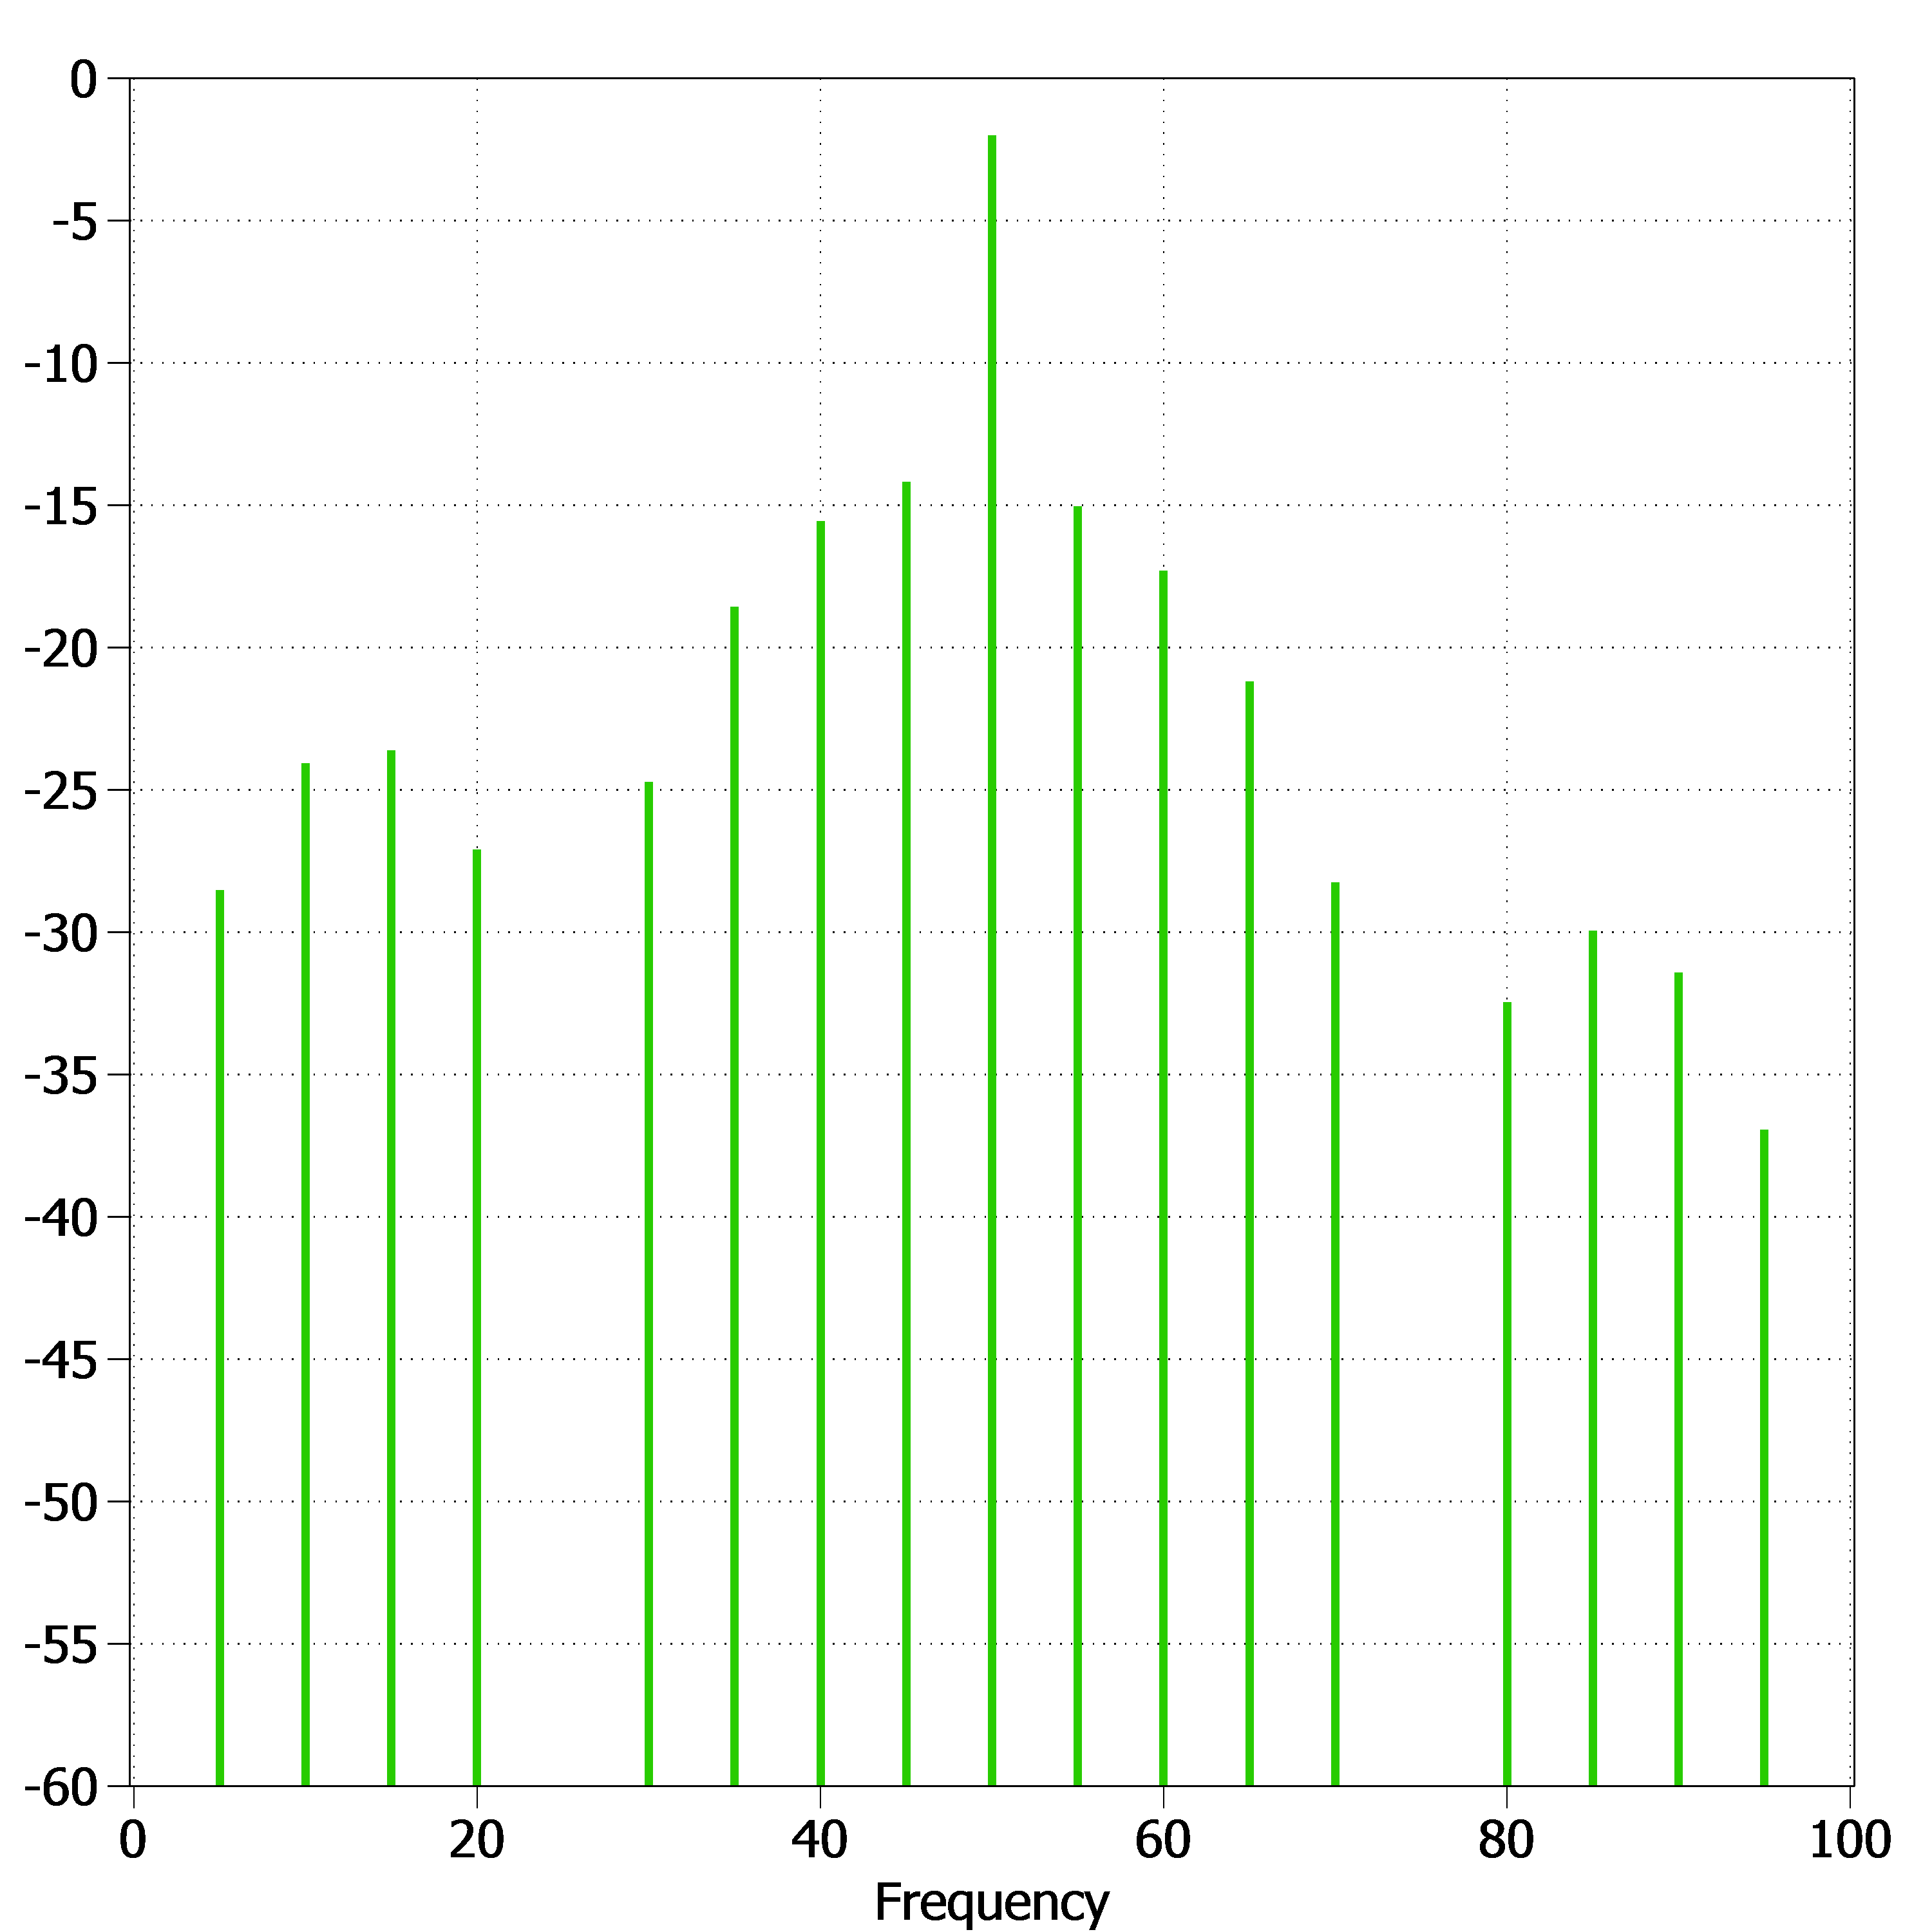
\includegraphics[width=0.45\linewidth]{plecs_schwingungspacket_0_8_absolut_log.PNG}\label{fig:plecs_Schwingungspaket_0_8_absolut_log}}
	\caption{Lineares absolutes Spektrum mit einem duty cycle von (a) 0.5 (b) 0.8}
	\label{fig:plecs_Schwingungspakete_absolut log}
\end{figure}

\subsubsection{Vergleich der einphasigen Resultate mit Plecs und Matlab}

Optisch betrachtet, sehen die Resultate der beiden einphasigen Simulationen sehr ähnlich aus. Um jedoch eine konkreten Bestätigung der Analyse zu erhalten, wurden alle Werte der einphasigen Simulationen nummerisch miteinander verglichen. Man erkannte, dass die meisten gegenübergestellten Werte eine Abweichung von unter 1 \% haben. Dies wurde als sehr niedrig empfunden. Somit konnten die beiden Simulationen auch nummerisch auf ihre Richtigkeit geprüft werden.  Alle Vergleiche, optisch und nummerisch sind im Anhang dargestellt.
\todo{Bilder in den Anhang schmeissen evt. no ei do ane}



\subsubsection*{dreiphasige Phasenanschnittsteuerung mit 60\textdegree und 90\textdegree}


Bei den folgenden Abbildungen \ref{fig:dreiphasige_Phasenanschnittsteuerung_mit_60} und \ref{fig:dreiphasige_Phasenanschnittsteuerung_mit_90} handelt es sich um die Simulation der dreiphasigen Phasenanschnittsteuerung, mit den bekannten Winkel von 60\textdegree  und 90\textdegree.
In den linken Bildern \ref{fig:3_phasiges_Phasenanschnitt_60_Signal} und \ref{fig:3_phasiges_Phasenanschnitt_90_Signal} ist im  unteren Bereich, dass Eingangssignal mit der verketteten Nennspannung von 400 Volt dargestellt. Die oberen Grafiken zeigen die Spannungen, welche über den Widerständen abfallen, nachdem der jeweilige Triac, mit dem eingestellten Winkel, gezündet hat. Die Werte der Widerstände stellte man auf 150 $\omega$ ein, da der Culatti im Messaufbau den gleichen Wert hat. Anhand von Cursor 1 erkennt man, dass zuerst eine positive Halbwelle der Eingangsspannung, des ersten Aussenleiter (grün), anliegt. Der positive Thyristor des ersten Triacs zündet somit bei 90\textdegree beziehungsweise bei 60\textdegree. Da der Sternpunkt bei dieser Schaltung nicht mit dem Neutralleiter verbunden wurde, tritt eine negative Spannung über dem Thyristor des zweiten Triac auf (rot). Beim Cursor 2 hat es eine negative Eingangsspannung des zweiten Aussenleiters (blau). Somit zündet der negative Thyristor des dritten Triacs und die entgegengesetzte positive Spannung ensteht über dem ersten Thyristor (grün) des ersten Triacs. Diese Abfolge wird beliebig weiter geführt. Da es sich nur um eine Ohmsche Last handelt, verhält sich das Stromsignal phasengleich wie die Spannungskurve. \\
Auf der Abbildung \ref{fig:3_phasiges_Phasenanschnitt_60_FTT} und \ref{fig:3_phasiges_Phasenanschnitt_90_FTT} erkennt man die beiden  FFTs der jeweiligen Phasenanschnittstuerungen. Es ist ersichtlich, dass auch bei dreiphasigen Phasenanschnittsteuerungen nur Harmonische Oberwellen vorkommen und keine Sub- oder Zwischenharmonische. 

\begin{figure}[ht!]
	\centering
	\subfloat[][]{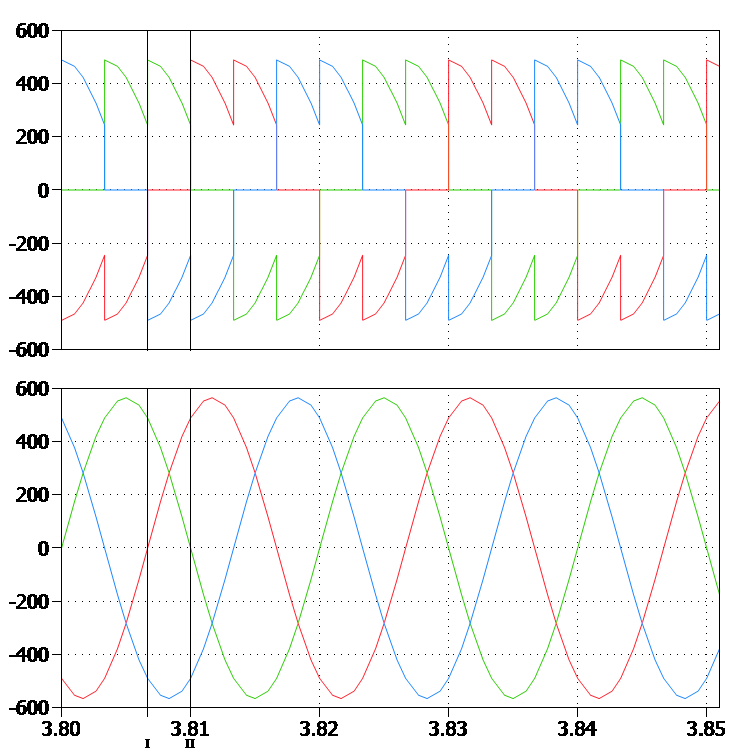
\includegraphics[width=0.45\linewidth]{3_phasiges_Phasenanschnit_60_Signal.png}\label{fig:3_phasiges_Phasenanschnitt_60_Signal}}\qquad
	\subfloat[][]{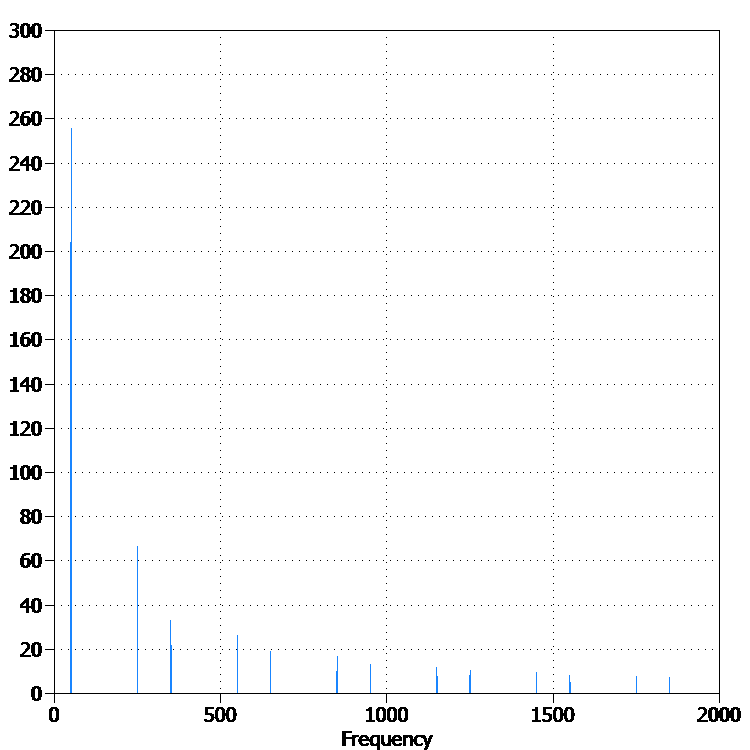
\includegraphics[width=0.45\linewidth]{3_phasiges_Phasenanschnit_60_FFT.png}\label{fig:3_phasiges_Phasenanschnitt_60_FTT}}
	\caption{dreiphasige Phasenanschnittsteuerung mit 60\textdegree (a) Signal (b) FFT}
	\label{fig:dreiphasige_Phasenanschnittsteuerung_mit_60}
\end{figure}

 

\begin{figure}[ht!]
	\centering
	\subfloat[][]{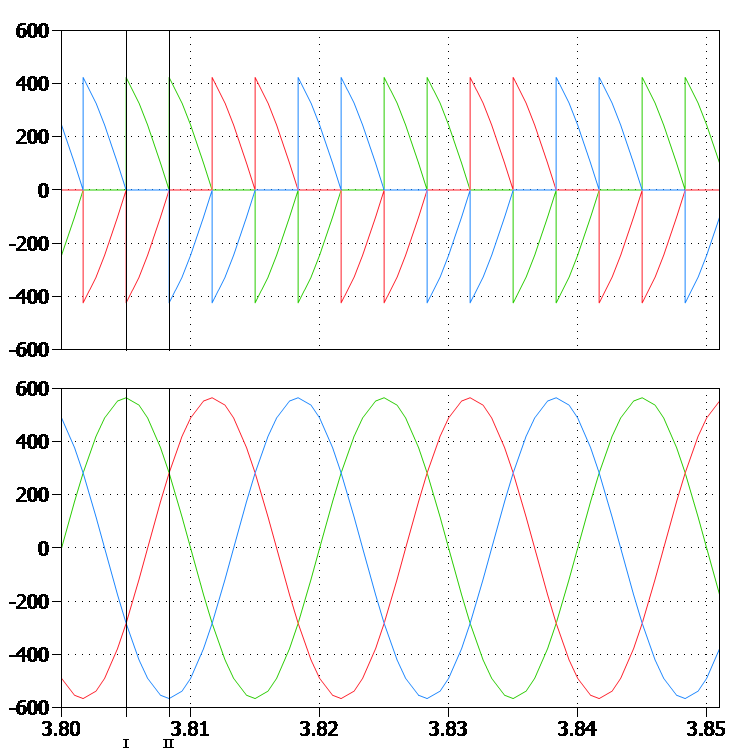
\includegraphics[width=0.45\linewidth]{3_phasiges_Phasenanschnit_90_Signal.png}\label{fig:3_phasiges_Phasenanschnitt_90_Signal}}\qquad
	\subfloat[][]{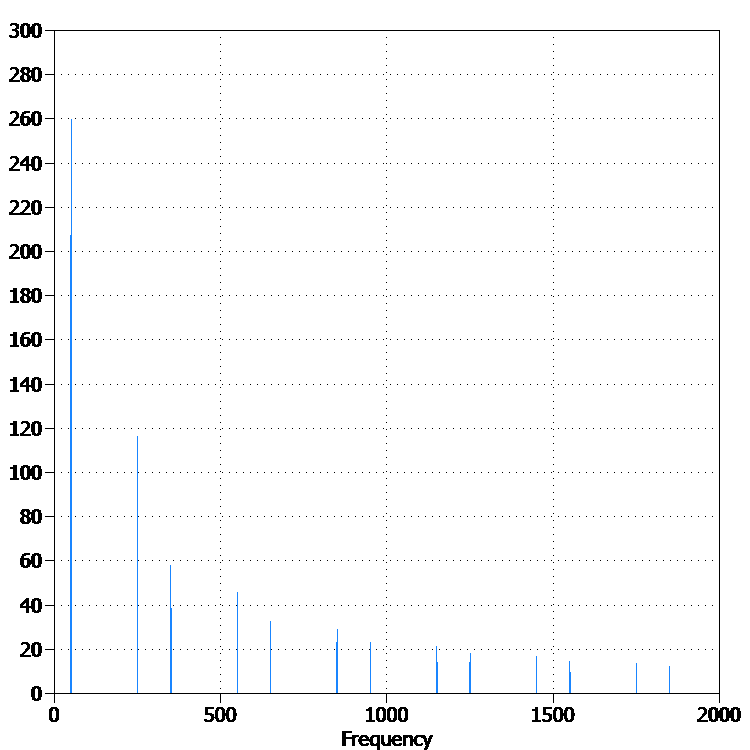
\includegraphics[width=0.45\linewidth]{3_phasiges_Phasenanschnit_90_FFT.png}\label{fig:3_phasiges_Phasenanschnitt_90_FTT}}
	\caption{dreiphasige Phasenanschnittsteuerung mit 90\textdegree (a) Signal (b) FFT}
	\label{fig:dreiphasige_Phasenanschnittsteuerung_mit_90}
\end{figure}



Nachfolgend sind die dreiphasigen Schwingungspaketsteuerungen mit den duty cycle von 0.5 in Abbildung \ref{fig:3_phasiges_Schwingungspaket_Signal_0_5} und 0.8 in Abbild \ref{fig:3_phasiges_Schwingungspaket_FTT_0_8} dargestellt. Die drei Eingangsspannungen und die Widerstände richtete man gleich, wie bei der dreiphasigen Phasenanschnittsteuerung, ein. Daher sind auch die Strom- und Spannungsverläufe wieder phasengleich. Bei den grünen, roten und blauen Kennlinien, handelt es sich um die Spannungspakete über den einzelnen Widerständen.\\
In den Bildern \ref{fig:3_phasiges_Schwingungspaket_FTT_0_5} und \ref{fig:3_phasiges_Schwingungspaket_Signal_0_8} sind die FFTs der Schwingungspaketsteuerung ersichtlich. Man erkennt vor allem, dass es vor und nach 50 Hz (hoher Peak) viele Sub- und Zwischenharmonische Oberschwingungen hat. Eine gewisse Ähnlichkeit mit den einphasigen Paketsteuerungen ist ersichtlich.
 

\begin{figure}[ht!]
	\centering
	\subfloat[][]{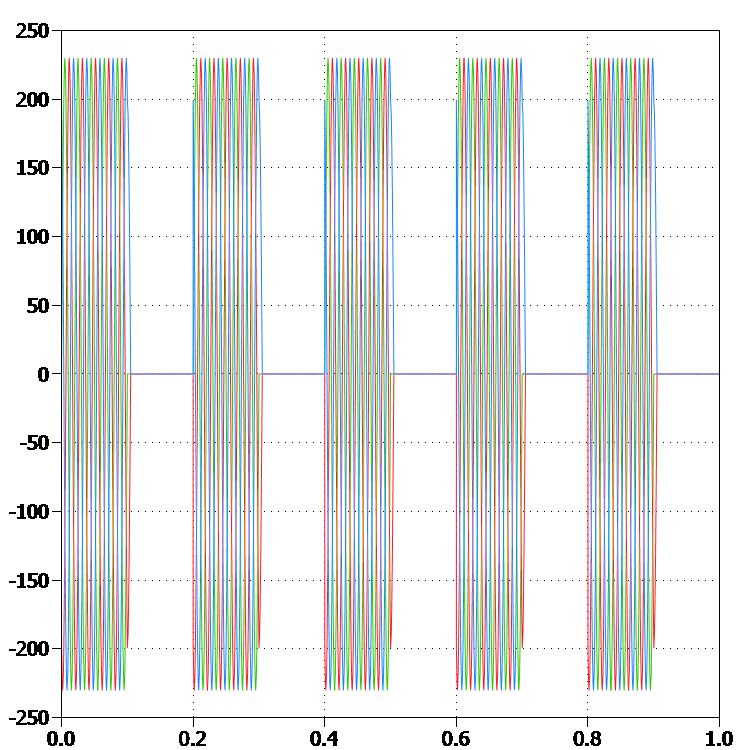
\includegraphics[width=0.45\linewidth]{3_phasiges_Schwingungspaket_Signal_0_5.png}\label{fig:3_phasiges_Schwingungspaket_Signal_0_5}}\qquad
	\subfloat[][]{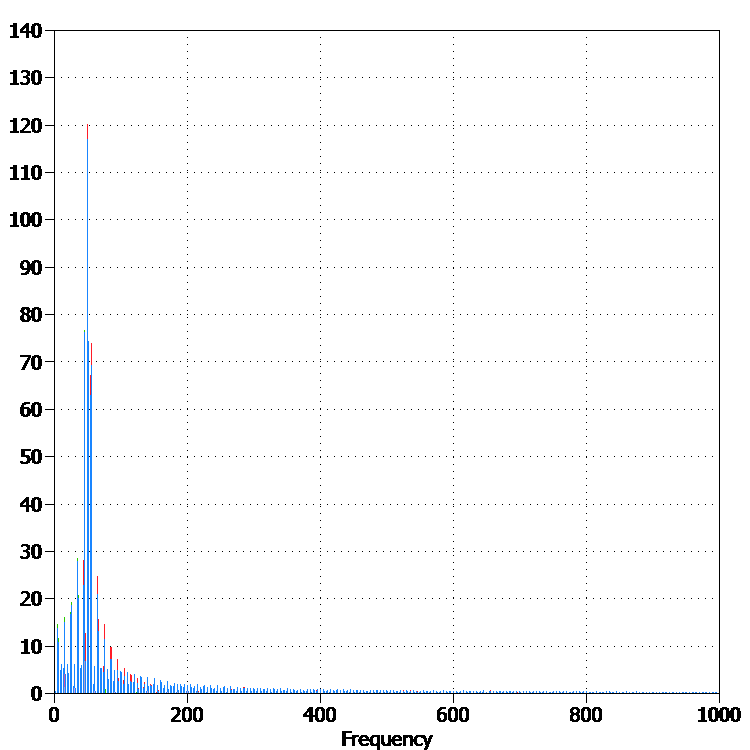
\includegraphics[width=0.45\linewidth]{3_phasiges_Schwingungspaket_FTT_0_5.png}\label{fig:3_phasiges_Schwingungspaket_FTT_0_5}}
	\caption{dreiphasige Schwingungspaketsteuerung mit duty cycle 0.5 (a) Signal (b) FFT}
	\label{fig:3_phasiges_Schwingungspaket_0_5}
\end{figure}


\begin{figure}[ht!]
	\centering
	\subfloat[][]{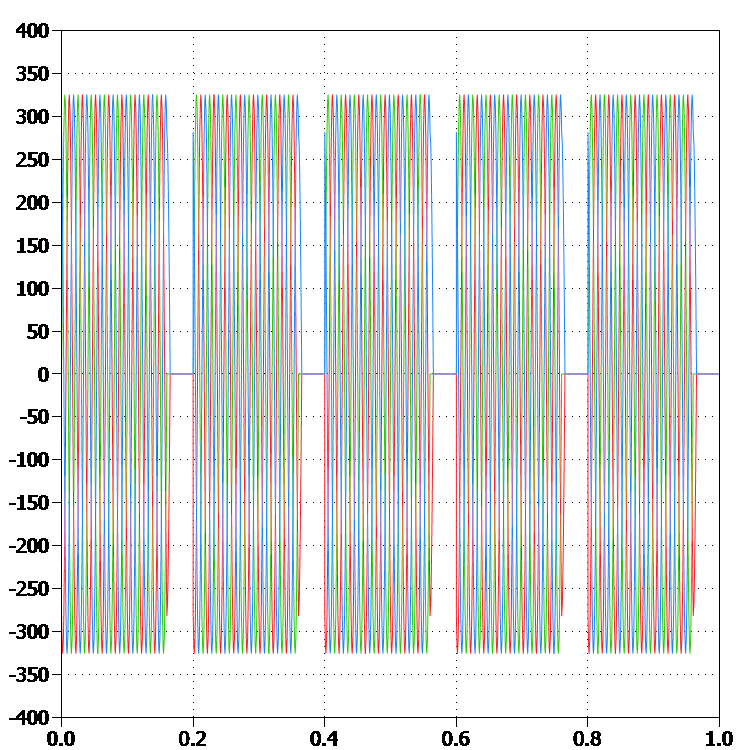
\includegraphics[width=0.45\linewidth]{3_phasiges_Schwingungspaket_Signal_0_8.png}\label{fig:3_phasiges_Schwingungspaket_Signal_0_8}}\qquad
	\subfloat[][]{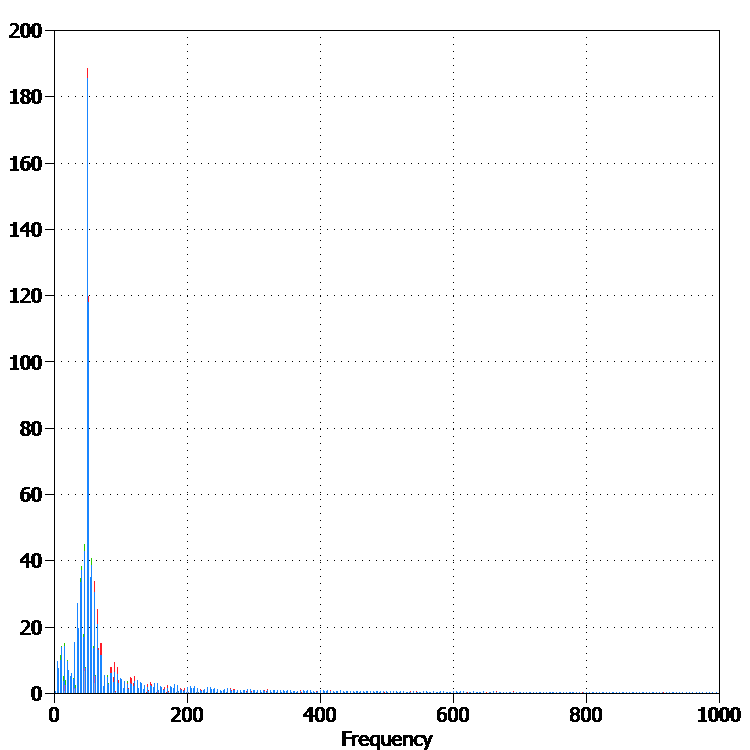
\includegraphics[width=0.45\linewidth]{3_phasiges_Schwingungspaket_FTT_0_8.png}\label{fig:3_phasiges_Schwingungspaket_FTT_0_8}}
	\caption{dreiphasige Schwingungspaketsteuerung mit duty cycle 0.8 (a) Signal (b) FFT}
	\label{fig:3_phasiges_Schwingungspaket_0_8}
\end{figure}

\newpage

\subsubsection{Alternative Ansteuerungen}
In der Praxis werden nicht immer alle 3 Phasen angesteuert, sogenannte Sparansteuerungen. Dabei können nur zwei oder auch nur eine Phase angesteuert werden. Das heisst, dass zum Beispiel bei der Zwei-Phasen-Ansteuerung bei einer Phase der Thyristor überbrückt wird beziehungsweise der Thyristor gar nicht vorhanden ist. Dabei dient die überbrückte Phase als Ausgleichs- und Rückleiter. Diese Fälle wurden mit Plecs simuliert wobei die Last in Stern und in Dreieck geschaltet werden kann. Wie bei der 3-Phasen Ansteuerung, wurde für die alternativen Ansteuerung auch der Sanft-Anlass, die Kombination mit Phasenanschnitts- und Schwingungspaketsteuerung, simuliert.

\subsubsection*{2-Phasen Ansteuerung mit Last in Stern}
\todo{Bild Simulation}

 
\subsubsection*{2-Phasen Ansteuerung mit Last in Dreieck}
\todo{Bild Simulation}


\subsubsection*{1-Phasen Ansteuerung mit Last in Stern}
\todo{Bild Simulation}


\subsubsection*{1-Phasen Ansteuerung mit Last in Dreieck}
\todo{Bild Simulation}


\subsubsection*{Halbwellensteuerung}
Eine weitere Möglichkeit, die Thyristoren anzusteuern, ist die Halbwellensteuerung. Dabei wird die positive Halbwelle einer Phasen und zwei negative Halbwellen der anderen Phasen auf die Last geführt. Dies ist mit dem Thyristorsteller, welcher für das Projekt benutzt wurde nicht möglich, da dieser alle 3 Phasen gleich ansteuert. Deshalb wurde dieser Fall nur mit Plecs simuliert. \todo{Einfügen Bild Simulation} Das Problem bei dieser Steuerung ist, dass wenn der Sternpunkt nicht mit dem Nullpunkt verbunden ist, der Phasenverlauf im Plecs schwer zu kontrollieren ist. Da die Summe der Spannungen immer 0 geben muss und die Spannungen phasenverschoben sind gibt es einen sehr unschönen Spannungsverlauf. Wenn das FFT analysiert wird, fällt schnell auf, das die Grundschwingung von 50 Hz nicht den höchsten Peak hat.



